\documentclass[conference]{IEEEtran}
\IEEEoverridecommandlockouts
% The preceding line is only needed to identify funding in the first footnote. If that is unneeded, please comment it out.
%\usepackage{cite}
\usepackage{amsmath,amssymb,amsfonts}
\usepackage{algorithm,algorithmic}
\usepackage{graphicx}
\usepackage{textcomp}
\usepackage{xcolor}
\usepackage{tabularx}
\usepackage{multirow}
\usepackage{caption}
\usepackage{subcaption}
\usepackage{fvextra}
\usepackage{bm}
\usepackage{pdfpages}
\usepackage{svg}

\def\BibTeX{{\rm B\kern-.05em{\sc i\kern-.025em b}\kern-.08em
    T\kern-.1667em\lower.7ex\hbox{E}\kern-.125emX}}
    
    
\newtheorem{definition}{Definition}
\newtheorem{theorem}{Theorem}
\newtheorem{example}{Example}

\newcommand\floorbrackets[1]{\ensuremath{%
		\bm{\lfloor}\mkern-1mu%
		\text{#1}%
		\bm{\rfloor}}}

\newcommand{\Attr}{\operatorname{attr}}
\newcommand{\Field}{\operatorname{field}}
\newcommand{\Values}{\mathbf{Values}}
\newcommand{\Token}{\mathbf{Token}}
\newcommand{\List}{\mathbf{List}}
\newcommand{\Sim}{\mathrm{sim}}
\newcommand{\Tokenize}{\mathbf{tokenize}}
    
    
    
    
    
    
    
    
    
    
    
    
    
    
    
    
\begin{document}

\title{
Accelerating Relational Keyword Queries With Embedded Neural Networks
}

\author{\IEEEauthorblockN{Limin Ma}
\IEEEauthorblockA{\textit{Faculty of Science} \\
\textit{Ontario Tech University}\\
Oshawa, Canada \\
limin.ma@ontariotechu.net}
\and
\IEEEauthorblockN{Ken Q. Pu}
\IEEEauthorblockA{\textit{Faculty of Science} \\
\textit{Ontario Tech University}\\
Oshawa, Canada \\
ken.pu@ontariotechu.net}
\and
\IEEEauthorblockN{Ying Zhu}
\IEEEauthorblockA{\textit{Faculty of Business and IT} \\
\textit{Ontario Tech University}\\
Oshawa, Canada \\
ying.zhu@ontariotechu.net}
}

\maketitle

\begin{abstract}
Relational keyword queries have proven to be highly effective for
information retrieval.  The challenge of evaluating keyword queries for
	relational databases is the performance bottleneck of fuzzy string
	matching when traditional full-text index structures.  We propose a
	solution to overcome performance bottlenecks by incorporating
	horizontally partitioned full-text indexes.  We rely on a neural
	network router to optimize the index lookup strategy to minimize index
	miss rate and thus maximize performance.  Using textural features of
	the user queries, the neural network router supports fuzzy string
	matching.  We evaluated different network architectural designs against
	real-world datasets.  Our experiments demostrates that the neural
	network router can be self-trained and learn how to optimize index
	access effectively.
\end{abstract}

\begin{IEEEkeywords}
keyword query, neural network, index structures
\end{IEEEkeywords}

\section{Introduction}


\section{Partial tuple search}
In this section, we formalize keyword queries as {\em partial tuple search}.
Let $R$ be a relational table.  Recall that $\Attr(R)$ is the attributes of $R$, and tuples in $R$ are mappings from $\Attr(R)$ to $\Values$.

\begin{definition}[Labeled values and partial tuple]
Let $R$ be a relational table.  A labeled value in $R$ is a pair $(l:x)$ where 
$l\in\Attr(R)\cup\{?\}$ and $x\in\Values$.  A partial tuple $\vec{x}$ is a set
of labeled values: $\vec x = \{(l_i, x_i): i\in I\}$.  We define the
attributes of a partial tuple $\vec x$ as the labels of the partial
tuple:
$$\Attr(\vec x) = \{l_i\}_{i\in I}$$.
A partial tuple is considered {\bf\em complete} if $\Attr(\vec x) = \Attr(R)$.
\end{definition}

We will write $\vec x[l_i]$ to denote the corresponding value $x_i$.

Note that a partial tuple is a set of values and their respective attribute
names from a relational table.  However, we allow a special symbol ``$?$" to be
in place of the attribute name.  The special attribute ``$?$" indicates that
the attribute name is unspecified (or unknown). The following example
illustrates two partial tuples. The second partial tuple has a wild card ``?"
as its attribute name:

\begin{example}
\begin{eqnarray*}
\vec s_1 &=& \{\mathrm{name}:\mathrm{Einstein}\} \\
\vec s_2 &=& \{\mathrm{name}:\mathrm{Einstein},\ \mathrm{?}: \mathrm{Professor}\}
\end{eqnarray*}
\end{example}

A keyword query is a partial tuple: $\vec Q = \{(l_i, q_i): i\in I_Q\}$.  The
values $q_i$ are keyword queries.
We want to find a complete tuple $\vec r \in R$ that matches $\vec Q$
optimally.  This requires us to define how to compare the partial tuple $\vec
Q$ with a complete tuple $\vec r$.  The guiding principle of comparing the two
tuples is to match labeled values from $\vec Q$ with those from $\vec r$
according to the following:
\begin{itemize}
    \item Match the labels if they are not the wild card ``$?$".
    \item Match the values using a fuzzy string matching score.
    \item Optimize the sum of similarities between labeled values from $\vec Q$ and those from $\vec r$.
\end{itemize}


\begin{definition}[Partial tuple search]
Let $R_1, R_2, R_3, \dots, R_K$ be $K$ relations. 
Given a user query that is a partial tuple: $$\vec Q = \{(l_i, q_i): i\in I_Q\}$$ 
where $l_i \in attr(R)\cup\{?\}$ and $q_i$ are keyword queries, 
we want to find a complete tuple $\vec r \in R_i,\ i\in\{1, 2, \dots, K\},$ that maximizes the similarity score
between the partial tuple $\Vec Q$ and full relational query $\vec r$.
\end{definition}

We use a neural network to optimize the query processing pipeline. Detailed
description can be found in  Section~\ref{sec:opt_pipeline}. We define the
neural network classifier as:

%\begin{definition}[Neural network classifier]
%Let $R_1, R_2, R_3, \dots, R_K$ be $K$ relations. The neural network classifier
%takes a partial tuple query $\vec q$ and estimates the probabilities
%that the search result of $\vec q$ belongs to relation $R_i$, $\forall
%i \in \{1, 2, \dots, K\}$.
%\end{definition}

\section{Partial tuple search using full-text search}
\label{sec:search_fulltext_index}
Traditional full-text indexes support keyword queries
over document collections using an inverted index data structure.  First the full relational
tuples are encoded as {\em documents} by some tokenizer.  The tokenizer breaks the string values of partial tuples
$\{q_i\}$ and full tuple $r\in R$ to {\em tokens}.  It's the comparison between $\mathbf{tokens}(q_i)$ and $\mathbf{tokens}(r)$
that determines their similarity.  To support approximate string matching, the standard approach \cite{kim2007n,kondrak2005n}
is to break down strings into their $n$-grams.  An example of a full-text encoding of a tuple is shown in Figure~\ref{fig:encoding}.

\begin{figure*}[t]
	\label{fig:encoding}
$$
\left[\begin{array}{rcl}
\mathrm{Name} & \mapsto & \makebox{\_\_J \_Ja Jac ack ck\_ k\_\_} \\
\mathrm{Address} & \mapsto & \makebox{\_\_1 \_10 100 00\_ 0\_\_ \_\_S \_Si Sim imc mco coe oe\_ e\_\_ \_\_S \_St Str tre ree eet et\_ t\_\_} \\
\mathrm{fulltext} & \mapsto & \makebox{\_\_J \_Ja Jac ack ck\_ k\_\_ \_\_1 \_10 100 00\_ 0\_\_ \_\_S \_Si Sim imc mco coe oe\_ e\_\_ \_\_S} \\ 
 & & \makebox{\_St Str tre ree eet et\_ t\_\_}\\
\end{array}\right]
$$
	\caption{Full text encoding of a relational tuple with 3-gram tokenization}
\end{figure*}

\section{Fuzzy keyword search with partitioned indexes}

Traditionally, a single full-text index is built on the tuples from all the relations. With the relations $\{R_1, R_2, \dots, R_n\}$, the aggregated index
is the full-text index built from the union of the tuples:
$$\mathbf{Index}_\mathrm{agg} = \textsc{InvertedList}\left(\bigcup_{i=1}^n R_i\right) $$

Due to the inverted list architecture, the performance bottleneck comes
from collisions of multiple documents containing the common tokens.  With the total number of document is given by $\sum_{i=1}^n |R_i|$, the average
number collision of the inverted lists in the aggregate index is estimated as:
$$
\mathbf{Collision}_\mathrm{agg} = \frac{
  \sum_{i=1}^n |R_i|
}{
  |\mathrm{vocab}|
}
$$
where $|\mathrm{vocab}|$ is the size of the vocabulary of the distinct tokens.
The query evaluate performance is known to be $\mathcal{O}(\mathbf{Collision})$.

When supporting fuzzy string matching, the tokenizer performs 3-gram tokenization,
and thus $\mathrm{vocab} = \makebox{all 3-grams} \in\mathcal{O}(1)$.  Namely,
with a fixed alphabet, the size of the vocabular is roughly a constant.  This means
the query evaluation time complexity is given by:

$$
\mathcal{O}(\mathrm{Lookup}(\mathbf{Index}_\mathrm{agg}, q)) = \mathcal{O}\left(\sum_{i=1}^n |R_i|\right)
$$

The query performance, thus, would degrade with increasing number of tuples, and increasing number of relations.

We propose the following strategies to overcome the performance bottleneck
of the aggregated index.

\begin{itemize}
\item We partition $\mathbf{Index}_\mathrm{agg}$ into multiple indexes
  $\{\mathbf{Index}_j: 1 \leq j \leq m\}$
\item Given a query $q$, we scan through the partitioned indexes
  and evaluate $\mathrm{Lookup}(\mathbf{Index}_j, q)$.
\end{itemize}

The advantages of the partitioned approach are:

\begin{itemize}
\item Each index access $\mathrm{Lookup}(\mathbf{Index}_j, q))$ is 
more {\em efficient} due to the reduced number of collisions in
the inverted index.

\item We have the opportunity of {\em optimizing} the sequence of scanning
the index partitions.  If we can determine the likelihood
of that the query $q$ has high similarity with tuples in $\mathbf{Index}_j$, we want
to access the partition $j$ before the other partitions.
\end{itemize}

\begin{algorithm}
	\label{alg:1}
\caption{Accelerated index lookup}
\begin{algorithmic}[1]
\REQUIRE $q$: Query, $partitions$: List of Partitions
\STATE $n \leftarrow$ length of $partitions$
\STATE $p$: List of float
\FOR{$i\in[0, n-1]$}
  \STATE $p[i] \leftarrow \mathbf{classifier}(q, partition[i])$
\ENDFOR
\FORALL{$i$ in sorted(range($n$), key=$\lambda$k: $p[k]$, desc)}
    \STATE $results \leftarrow$ Lookup($partitions[i]$, $q$)
    \STATE yield $results$
\ENDFOR
\end{algorithmic}
\end{algorithm}

In Algorithm~\ref{alg:1}, it evaluates the probability of if $q$
is relevant to the tuples in the $i$th partition.  The probability
is computed as a binary classifier 
$$\mathbf{classifier}(\mathbf{Index}, \mathbf{Query})$$

\section{Design and training of classifiers}

Each index partition has an accompanying binary classifier $\mathbf{Classifier}_i : \mathbf{Query}\to[0, 1]$.
We use a neural network to learn the classification function.  Due to the application
scenario, the design constraints are:

\begin{itemize}
\item The neural network must be compact in size so that they can be embedded in
	the database runtime system.  Our goal is that the neural network is a small
	memory addition to the keyword query evaluation engine.
\item The inference speed of the neural network incurs a minimal overhead.  This means
	we prefer shallow networks over deeper architectures.
\end{itemize}

\subsection{Vectorization of tokens and queries}

\noindent{\bf Token representation of queries}:  given a query $\vec q=\{(l_i,
x_i): 1\leq i \leq m\}$, we generate the text representation of the query by
simply concatenating the text representation of labels and the tokenized query
values.
\begin{eqnarray*}
	\mathbf{tokens}(\vec q) &=& \{l_1\} \oplus \mathbf{tokenize}(x_1)  \\
				&&  \oplus \{l_2\} \oplus \mathbf{tokenize}(x_2) \\
				&& \oplus \dots \{l_m\} \cup \mathbf{tokenize}(x_m)
\end{eqnarray*}
where $\oplus$ is sequence concatenation.

\noindent{\bf Integer encoding of queries}: next we encode $\mathbf{tokens}(\vec q)$ using a universal
vocabulary $\mathbf{vocab}$.  The vocabulary consists of all known tokens, and their respective
ordinal integer code.  This vocabulary will be built using the existing relational tuples.  The construction of the vocabulary is described in subsequent sections.  The vocabulary is described as a function from tokens to integers:
$$ \mathbf{vocab} : \mathbf{Token} \to \mathbb{N}$$

The integer sequence of a query is given by:
$$
\mathbf{sequence}(\vec q) = \mathbf{vocab}\circ\mathbf{tokens} (\vec q) \in\mathbb{N}^*
$$

\noindent{\bf Embedding vectors of queries}:
Using a standard embedding layer (Section~\ref{sec:embedding-layer}), embed the integer sequence representation of the query
to a sequence of latent vectors.

$$
\mathbf{vector}(\vec q) = \mathbf{Emb}(\mathbf{sequence}(\vec q))\in\mathbb{R}^{|q|\times d}
$$

At this point, we have many options in mapping
the vector sequence to the probability distribution
in $\mathbb{R}^n$.


% -------------------------------------------------------------------------------
% XXX
\vspace{2cm}

\noindent\makebox[\linewidth]{\rule{0.5\textwidth}{5pt}}

\vspace{2cm}
% -------------------------------------------------------------------------------



For the remainder of this chapter, we denote the vector sequence representation of $\vec q$ as:

$$\vec x = \mathbf{sequence}(\vec q) = (x_1, x_2, \dots, x_{|q|})$$
where each $x_i\in\mathbb{R}^d$ is the embedding vector 
of the $i$-th token in a $d$-dimensional latent space.

\subsection{Neural network architectures for query classification}
\label{sec:architectures}

\noindent{\bf MLP based classification}.

Given the input of vectorized query representation $\vec x$, 
we first flatten it using global average over the entire sequence length.  Then, we process it with a MLP with softmax
activation function.  The MLP must have $n$ output neurons.

$$
\begin{array}{rlr}
&\vec x  & (|q|, d) \\
\to & \left(\frac{\sum_{i=1}^{|q|} x_i}{|q|}\right) & (d) \\
\to & \mathbf{MLP}(\makebox{output-dim}=n) & (n) \\
\to & \mathbf{softmax}(\cdot) & (n) \\
\end{array}
$$

\noindent{\bf Recurrent network architecture with LSTM cells}.

Since recurrent neural networks (RNN) are specifically designed to process sequence inputs, we can utilize
a RNN to map the input $\vec x$ to a flattened state vector, which can then be processed
by a MLP to compute the output probability distribution.

The advantage of RNN is that it can learn inter-token dependencies in the query at the cost of
a bigger model size and higher training cost.

$$
\begin{array}{rlr}
&\vec x  & (|q|, d) \\
\to & \mathbf{LSTM}(\makebox{output-state=True}) & (d) \\
\to & \mathbf{MLP}(\makebox{output-dim}=n) & (n) \\
\to & \mathbf{softmax}(\cdot) & (n) \\
\end{array}
$$

\noindent{\bf 1D convolution architecture}.

Another standard technique to learn sequential features is to use 1D convolution.
The 1D convolution layer (Section~\ref{sec:cnn}) produces a sequence of {\em feature} vectors
that capture the short-range token dependencies within the convolution window size.  We then use
global averaging to flatten the convolution features for further processing using a MLP.

$$
\begin{array}{rlr}
&\vec x  & (|q|, d) \\
\to & \mathbf{Conv1D} & (|q|, d) \\
\to & \mathbf{Global\ Average} & (d)\\
\to & \mathbf{MLP}(\makebox{output-dim}=n) & (n) \\
\to & \mathbf{softmax}(\cdot) & (n) \\
\end{array}
$$

\noindent{\bf Transformer and MLP Mixer}

Transformers have shown to be a superior architecture for many tasks in the domain of MLP and sequence learning.  The exact architecture of a transformer block is shown in the implementation section (See Figure~\ref{fig:transformer_model}).  Due to the nature of our problem, we chose to use only a single transformer block so that the model remains small enough to be embedded in the query processing pipeline.

A more recent MLP based architecture is MLP mixer which is a concatenation of two MLP layers separated by a matrix transpose operation.  Details of the MLP mixer are shown in Figure~\ref{fig:mlpmixer_model}.

\subsection{Unsupervised training of neural network classifiers}

The classifier needs to be trained with data of the following form:
$$
(\vec q, i)
$$
where $\vec q$ is a sample query, and $i$ is the relation $R_i$ that contains the best matching
tuple of $\vec q$.

The training data is generated directly from the relational tuples from the database.  For each complete tuple $\vec r = \{(l_i, x_i): i\in I\}$, we formed a query $\vec q_r$ by random sampling from
the labeled values while masking the labels.

$$
\vec q_r = \{(?, x_i): i\in\mathbf{sample}(I)\}
$$

Thus, given a database with $n$ relations $R_1, R_2, \dots, R_n$:
$$
\mathbf{train} = \bigcup_{i=1}^n\{(\vec q_r, i): r\in R_i\}
$$

\section{Overall query processing pipeline}

To summarize the proposed query processing pipeline for partial tuple search, we have the following stages:

\begin{enumerate}
    \item A partial tuple is entered as user input.
    \item The partial tuple is tokenized and converted to a structured keyword query.
    \item The neural network classifier sorts the partitioned indexes based on the probability scores.
    \item The partitioned indexes are scanned to find top-$k$ complete tuple candidates from the database.
    \item The candidates are ranked by max-matching based similarity scores.
\end{enumerate}

Our pipeline requires that partitioned full-text indexes are built from tuples of each relation in offline mode. In addition, the neural network classifier should be trained using sampled tuples from each relation.




% ---------------------------------------------------------












\section{Experimental Evaluation}

In this section, we will describe the evaluation of the proposed solutions.  We will verify the effectiveness and limitations of our solutions, and perform a comparative study of different network architectures.  For each network architecture, we will present the benefits and drawbacks, and provide our understanding of the explanation of the observations.

\subsection{Datasets}
The datasets we have used to evaluate our system is a collection of survey data from Statistics Canada \cite{ds01, ds02, ds03, ds04, ds05, ds06, ds07, ds08, ds09, ds10}, which includes one labour force survey, six COVID-19 surveys, one income survey, one community health survey, and one housing survey.
They offer many real-world characteristics that pose as challenges to  neural network classifiers.  Given the intended application scenarios of our research, we felt that it was important to evaluate our work using real-world datasets. For easy reference in subsequent sections, we give each dataset an id, as shown in Table \ref{table:id_name}.   
\begin{table}[t]
	\centering
	\begin{tabularx}{\textwidth}{|l|X|}
		\hline
		\textbf{Dataset id} & \textbf{Dataset name} \\
		\hline
		ds01 & Labour Force Survey, April 2019 [Canada] \\
		ds02 & Crowdsourcing: Impacts of COVID-19 on Canadians’ Experiences of Discrimination Public Use Microdata File \\
		ds03 & Crowdsourcing: Impacts of COVID-19 on Canadians Public Use Microdata File, [2020] \\
		ds04 & Crowdsourcing: Impacts of the COVID-19 on Canadians – Your Mental Health Public Use Microdata File, [2020] \\
		ds05 & Crowdsourcing: Impacts of COVID-19 on Canadians' Perception of Safety Public Use Microdata File, [2020] \\
		ds06 & Crowdsourcing: Impacts of the COVID-19 on Canadians – Trust in Others Public Use Microdata File [2020] \\
		ds07 & Impacts of the COVID-19 pandemic on postsecondary students (ICPPS) 2020, Crowdsource file, Public use microdata file \\
		ds08 & Canadian Income Survey (CIS), 2017 \\
		ds09 & Canadian Community Health Survey - Annual Component (CCHS) 2017-2018 \\
		ds10 & Canadian Housing Survey, 2018 \\
		\hline
	\end{tabularx}
	\caption{Dataset ids and names}
	\label{table:id_name}
\end{table}

These 10 datasets contain both numerical and textual data with different numbers of attributes and tuples. For example, the labour force survey contains data of the Canadian labour market. It has total 60 attributes related to the job market, such as employment status, industry, status of working full-time or part-time, hourly wage, etc. Table \ref{tab:ds01_samples} shows 5 samples with a subset of 10 attributes. The descriptions of the selected 10 attributes are shown in table \ref{tab:ds01_attrs_samples}.
\begin{table}[!ht]
	\centering
	\resizebox{\textwidth}{!}{%
		\begin{tabular}{
				|c
				|c
				|>{\raggedright\arraybackslash}p{0.1\textwidth}
				|>{\raggedright\arraybackslash}p{0.1\textwidth}
				|l
				|>{\raggedright\arraybackslash}p{0.2\textwidth}
				|>{\raggedright\arraybackslash}p{0.2\textwidth}
				|>{\raggedright\arraybackslash}p{0.2\textwidth}
				|l
				|l|}    \hline
			\multicolumn{1}{|c|}{\textbf{survyear}} &
			\multicolumn{1}{c|}{\textbf{survmnth}} &
			\multicolumn{1}{c|}{\textbf{lfsstat}} &
			\multicolumn{1}{c|}{\textbf{prov}} &
			\multicolumn{1}{c|}{\textbf{age\_12}} &
			\multicolumn{1}{c|}{\textbf{educ}} &
			\multicolumn{1}{c|}{\textbf{immig}} &
			\multicolumn{1}{c|}{\textbf{noc\_10}} &
			\multicolumn{1}{c|}{\textbf{ftptmain}} &
			\multicolumn{1}{c|}{\textbf{hrlyearn}} \\ \hline
			2019 &
			April &
			Employed, at work &
			Ontario &
			25 to 29 years &
			Postsecondary certificate or diploma &
			Non-immigrant &
			Natural resources, agriculture and related production occupations &
			Full-time &
			33.00 \\
			2019 &
			April &
			Not in labour force &
			British Columbia &
			70 and over &
			Bachelors degree &
			Non-immigrant &
			&
			&
			\\
			2019 &
			April &
			Employed, at work &
			British Columbia &
			45 to 49 years &
			High school graduate &
			Non-immigrant &
			Business, finance and administration occupations &
			Full-time &
			26.00 \\
			2019 &
			April &
			Employed, at work &
			Ontario &
			20 to 24 years &
			Postsecondary certificate or diploma &
			Non-immigrant &
			Health occupations &
			Full-time &
			37.60 \\
			2019 &
			April &
			Employed, at work &
			Ontario &
			70 and over &
			Some postsecondary &
			Immigrant, landed more than 10 years earlier &
			Occupations in art, culture, recreation and sport &
			Part-time &
			32.00 \\ \hline
		\end{tabular}%
	}
	\caption{5 samples from the labour force survey dataset ``ds01", showing only 10 attributes.}
	\label{tab:ds01_samples}
\end{table}
\begin{table}[t]
	\centering
	\begin{tabular}{|l|l|}
		\hline
		\multicolumn{1}{|c|}{\textbf{Attribute}} & \multicolumn{1}{c|}{\textbf{Description}}     \\ \hline
		survyear & Survey year                        \\
		survmnth & Survey month                       \\
		lfsstat  & Labour force status                \\
		prov     & Province                           \\
		age\_12  & Five-year age group of respondent  \\
		educ     & Highest educational attainment     \\
		immig    & Immigration status                 \\
		noc\_10  & 2016 NOC (10 categories)           \\
		ftptmain                                 & Full- or part-time status at main or only job \\
		hrlyearn & Usual hourly wages, employees only \\ \hline
	\end{tabular}
	\caption{10 attributes and their descriptions from the labour force survey dataset ``ds01".}
	\label{tab:ds01_attrs_samples}
\end{table}
Table \ref{table:ds_stats} shows the number of attributes and tuples in each dataset.
\begin{table}[t]
	\centering
	\begin{tabular}{ |l|r|r|r|r|r|r|r|r|r|r| }
		\hline
		\textbf{Dataset id} & \textbf{No. of attrs.} & \textbf{No. of tuples} \\
		\hline
		ds01 & 60 & 100,885 \\
		ds02 & 129 & 36,662 \\
		ds03 & 47 & 242,512 \\
		ds04 & 43 & 45,989 \\
		ds05 & 23 & 43,631 \\
		ds06 & 47 & 36,538 \\
		ds07 & 42 & 101,902 \\
		ds08 & 194 & 92,286 \\
		ds09 & 1051 & 113,286 \\
		ds10 & 132 & 61,750 \\
		\hline
	\end{tabular}
	\caption{Number of attributes and tuples in each dataset.}
	\label{table:ds_stats}
\end{table}

Sometimes different datasets share common attributes. For example, the COVID-19 datasets have a common attribute about community size and metropolitan influence zones where the survey correspondents live in. By using multiple partial tuple completion, users can ``jump" from one dataset to another. For example, users may find some data related to discrimination from the dataset of impacts of COVID-19 on Canadians’ experiences of discrimination. Then they can use the results to search more information about people's perception of safety in the communities with the same sizes in the dataset of impacts of COVID-19 on Canadians’ perception of safety. This will help users to gain more insights from the survey results.

\section{Architecture and software stack}
In order to thoroughly evaluate the end-to-end search system, we have developed a platform with the following technology stack.  We use Lucene \cite{lucene} as the full-text index.  A customized search engine is developed on top of Lucene to support partial tuple search queries.  This is necessary for us to have detailed instrumentation to collect performance metrics, and to gain control over the ordering of text index search.  We have implemented all neural network based classifiers using TensorFlow \cite{tensorflow}. The trained models are used to generate the ordering of Lucene index access. 
The evaluation of the neural network acceleration is based on the speed-up of query performance between the machine learning generated ordering and other alternatives.
In addition, top-$k$ accuracy is also used to evaluate models.
The query workloads used in evaluation are generated from the datasets themselves. Figure \ref{fig:proj_arch} shows the high-level architectural overview of our implementation. More details about the training datasets and the query workload generation will be presented in subsequent sections.
\begin{figure}[!th]
	\centering
%	\includesvg[inkscapelatex=false, width = 250pt]{overall_architecture.svg}
	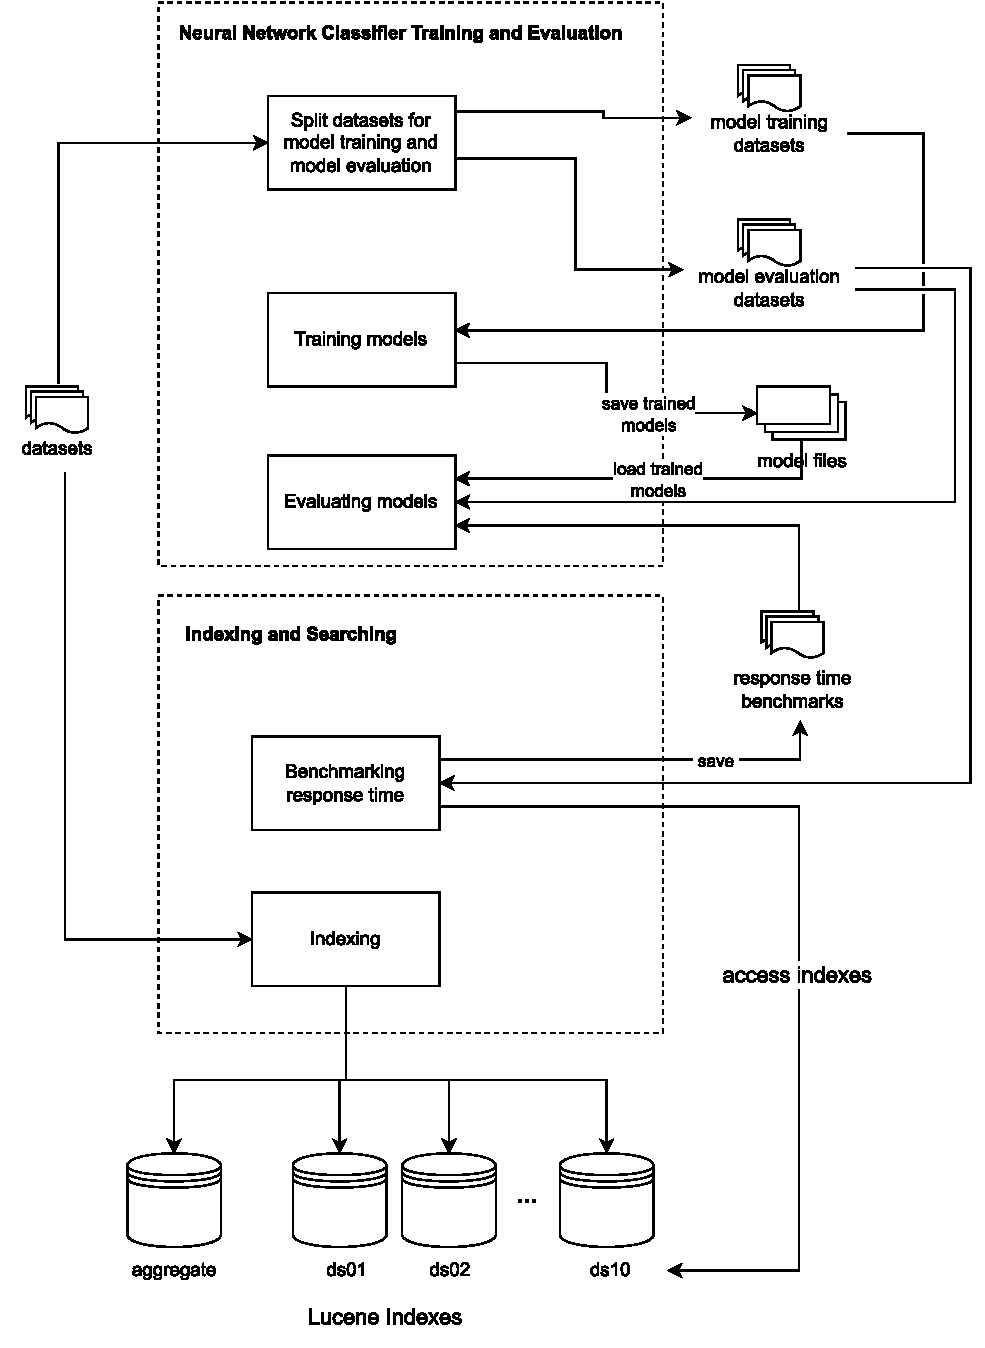
\includegraphics[width=0.8\textwidth]{graphics/overall_architecture.pdf}
	\caption{High-level overview of architecture}
	\label{fig:proj_arch}
\end{figure}

\subsection{Lucene and a customized search engine}
We developed a customized search engine on top of Lucene. It has two main functions. The first is to index datasets to create Lucene indexes. 
When indexing datasets, each tuple is converted to a Lucene document, which contains a set of \emph{(attribute name, attribute value)} pairs. We apply character-based 3-gram tokenization to attribute values. We use the special character ``\_" for padding. In addition, we add an extra field ``fulltext" to the document, which contains all 3-gram tokens of all attribute values. This field is needed to support full-text search.
For example, given a tuple $t$ as, 
$$
\{\mathrm{Name}:Jack,\ \mathrm{Gender}:Male,\ \mathrm{Occupation}:\makebox{Software developer}\}
$$
our search engine will first apply Lucene's standard tokenization, and then our character-based 3-gram tokenization. The resulting Lucene document will be,
$$
\left[\begin{array}{rl}
\mathrm{name}: & \_\_j\ \_ja\ jac\ ack\ ck\_\ k\_\_ \\
\mathrm{gender}: & \_\_m\ \_ma\ mal\ ale\ le\_\ e\_\_ \\
\mathrm{occupation}: & \_\_s\ \_so\ sof\ oft\ ftw\ twa\ war\ are\ re\_\ e\_\_\ \_\_d\ \_de\ dev\ eve\ vel \\
& elo\ lop\ ope\ per\ er\_\ r\_\_ \\
\mathrm{fulltext}: & \_\_j\ \_ja\ jac\ ack\ ck\_\ k\_\_\ \_\_m\ \_ma\ mal\ ale\ le\_\ e\_\_\ \_\_s\ \_so\ sof \\
& oft\ ftw\ twa\ war\ are\ re\_\ e\_\_\ \_\_d\ \_de\ dev\ eve\ vel\ elo\ lop\ ope \\
& per\ er\_\ r\_\_
\end{array}\right]
$$

The second main function is to support partial tuple search queries. We also use character-based 3-gram tokenization when constructing a search query. For example, given a partial tuple as:
$$
\{\mathrm{Name}:Jack,\ \mathrm{Gender}:Male\}
$$
the search query will be:
$$
\{\mathrm{fulltext}: \_\_j\ \_ja\ jac\ ack\ ck\_\ k\_\_\ \_\_m\ \_ma\ mal\ ale\ le\_\ e\_\_\}
$$

\subsection{Partitioned indexes and an aggregate index}

We have indexed the tuples from all datasets into a single Lucene index.  The tuples are tokenized  using the 3-gram tokenizer in order to support fuzzy string matching as described in Section~\ref{sec:fuzzy-collision}.  This index will be referred to as the {\em aggregate index} since it contains all the tuples from 10 datasets in a single index.  The aggregate index contains approximately 877,000 documents.

We also have an alternative way of indexing the tuples using Lucene.  We partition the tuples based on which relation they belong to.  Given that we have 10 datasets, we have created 10 individual indexes, each containing the tuples from their respective relation.  We refer to the set of indexes as {\em partitioned indexes}.
The number of documents in each partitioned index is the same as the number of tuples in each dataset, as shown in Table \ref{table:ds_stats}.

With the two types of indexing schemes (partitioned vs aggregate indexing), we have many alternatives in evaluating a user query.

\noindent {\bf Aggregate index lookup:} we can simply issue the user query against the aggregate index as it contains all the available tuples.  

\begin{itemize}
    \item Pro: This is the traditional approach. It requires the least system design. Only a single thread is needed for each user query.
    \item Con: As we have indicated previously and will show in our experimental evaluation, this approach suffers from a performance bottleneck resulting from high token hashing collision rate.
\end{itemize}

\noindent {\bf Parallel lookup of partitioned indexes:} we can issue the query against all individual index in the partitioned index set.  This will perform parallel index lookup using multiple concurrent threads.

\begin{itemize}
    \item Pro: The result can be found quickly.  The index with the {\em correct} tuple will contain much less documents compared to the aggregate index, and thus will respond with the search result faster.  In fact, we argue that this is the optimal performance one can expect.
    \item Con: The concurrency will impose a higher CPU and disk IO demand as each user query will take up to $n$ threads to process.  In high traffic or low resource scenarios, this may be prohibitively expensive.
\end{itemize}

{\noindent \bf Predictive sequential lookup of partitioned indexes}: we advocate to perform single threaded  access of the partitioned indexes.  But rather than simple or random sequential scan of the index set, we utilize predictive neural networks to generate an optimized access pattern, as described in Section~\ref{sec:opt_pipeline}.

\begin{itemize}
    \item Pro: This method enjoys the advantage of both single-threaded index lookup and  low disk latency due to the potential early hit in a smaller partitioned index.  So we argue that the predictive lookup will yield high query performance and low resource usage.
    \item Con: This method requires a self-supervised neural network to perform the prediction.
\end{itemize}

\section{Evaluation methodology}
We evaluate five model architectures, including Multilayer Perceptron (MLP), Long Short-Term Memory (LSTM), 1D Convolution (Conv1D), Transformer and MLP-Mixer. We also exam how misspelled keywords affect the models' top-5 accuracies.

We use two metrics for model evaluation. The first metric is query processing time. We submit queries to partitioned indexes and the aggregate index, and record the response times as evaluation benchmark. More details are given in the subsection \ref{subsection:perf_baseline_expt}.

The second metric is top-$k$ accuracy. A model's prediction gives us the ordering of Lucene index access. If the Lucene index that a query belongs to is among the top-$k$ of the model's prediction, we consider the prediction accurate. For example, for a query sampled from \verb|ds02|, if the predicted access ordering is 
\begin{verbatim}
idx_ds06, idx_ds10, idx_ds07, idx_ds05, idx_ds02, ...
\end{verbatim}
we consider it an accurate top-5 prediction.

In the following subsections, we give more details about our training data, query workloads and experiments. We first describe how training data and query workloads are generated and tokenized in subsections \ref{subsection:training_data_gen} and \ref{subsection:query_workload_gen}, respectively. 
After that, we describe our experiments in subsections starting from  \ref{subsection:perf_baseline_expt} to  \ref{subsection:expt_3gram_resiliency}.

\subsection{Training data generation and tokenization}
\label{subsection:training_data_gen}
The raw datasets are in SAS7BDAT format, which is a binary database format. To make data processing easier for the downstream model training and evaluation, we convert all raw datasets to CSV files. Then we remove some unuseful attributes. For example, the labour force survey dataset contains the attribute \emph{rec\_num}, which indicates the record number in the file. This attribute is removed since it is not useful for our model training. After that the preprocessed CSV files are splitted into data for model training and data for model evaluation. Data for model evaluation are used to generate query workloads. More details about the query workloads generation will be presented in subsection \ref{subsection:query_workload_gen}.

Our next step is to generate training datasets from data reserved for model training. We randomly sample tuples from each CSV file without replacement. Then we normalize the sampled tuples to lowercase and remove special characters from them, which gives us word-based training data. In addition, we also apply character-based 3-gram tokenization to normalized tuples. We use ``\_" as the special character for padding in our implementation.  This results in 3-gram based training data. For example, given a raw tuple:
\begin{verbatim}
(2019,April,"Employed, at work",Nova Scotia,Other CMA or non-CMA,
45 to 49 years,,Female,Married,Above bachelor''s degree,
"Single jobholder")
\end{verbatim}
the normalized tuple will be:
\begin{verbatim}
(2019,april,employed at work,nova scotia,other cma or non cma,
45 to 49 years,female,married,above bachelors degree,
single jobholder)
\end{verbatim}
and the 3-gram tokenized tuple will be:
\begin{verbatim}
(__2 _20 201 019 19_ 9__,__a _ap apr pri ril il_ l__,__e _em emp mpl
plo loy oye yed ed_ d__ __a _at at_ t__ __w _wo wor ork rk_ k__,__n 
_no nov ova va_ a__ __s _sc sco cot oti tia ia_ a__,__o _ot oth the 
her er_ r__ __c _cm cma ma_ a__ __o _or or_ r__ __n _no non on_ n__ 
__c _cm cma ma_ a__,__4 _45 45_ 5__ __t _to to_ o__ __4 _49 49_ 9__ 
__y _ye yea ear ars rs_ s__,__f _fe fem ema mal ale le_ e__, __m _ma
mar arr rri rie ied ed_ d__,__a _ab abo bov ove ve_ e__ __b _ba bac
ach che hel elo lor ors rs_ s__ __d _de deg egr gre ree ee_ e__,__s
_si sin ing ngl gle le_ e__ __j _jo job obh bho hol old lde der er_
r__)
\end{verbatim}
Since we evaluate our models using partial tuple queries, a natural question is whether training models using partial tuples will have any impact on models' performance. Therefore, besides training datasets containing full tuples, we also create datasets containing partial tuples with 75\% and 50\% of attributes. Since each dataset will have an additional 3-gram tokenzed version, we have total six sets of training datasets. Table \ref{tab:training_vocab_size} shows their vocabulary sizes. In addition, we use dataset names as labels, so there is no need to manually label training tuples.
\begin{table}[t]
	\centering
	\resizebox{\textwidth}{!}{%
		\begin{tabular}{|l|ll|ll|ll|}
			\hline
			\multirow{2}{*}{\textbf{}} &
			\multicolumn{2}{c|}{\textbf{100\% attrs.}} &
			\multicolumn{2}{c|}{\textbf{75\% attrs.}} &
			\multicolumn{2}{c|}{\textbf{50\% attrs.}} \\ \cline{2-7} 
			&
			\multicolumn{1}{l|}{word-based} &
			3-gram based &
			\multicolumn{1}{l|}{word-based} &
			3-gram based &
			\multicolumn{1}{l|}{word-based} &
			3-gram based \\ \hline
			\multicolumn{1}{|c|}{vocabulary size} &
			\multicolumn{1}{r|}{56,482} &
			\multicolumn{1}{r|}{4,136} &
			\multicolumn{1}{r|}{47,536} &
			\multicolumn{1}{r|}{4,130} &
			\multicolumn{1}{r|}{37,183} &
			\multicolumn{1}{r|}{4,109} \\ \hline
		\end{tabular}%
	}
	\caption{Vocabulary size of six sets of training datasets.}
	\label{tab:training_vocab_size}
\end{table}

\subsection{Query workload generation and tokenization}
\label{subsection:query_workload_gen}
Query workloads are sets of partial tuples. 
We first randomly sample tuples from data reserved for model evaluation. 
Then we apply the same normalization process to them as we do to training datasets. 
After that we convert them to partial tuples by randomly sampling some attributes from them.
We create different workloads by varying the number of attributes sampled.
Table \ref{tab:workloads} shows two query workloads we used for model evaluation.
\begin{table}[t]
	\centering
	\begin{tabularx}{0.8\textwidth}{|l|X|}
		\hline
		\textbf{Workload name} & \textbf{Description} \\ \hline
		workload A & 5 randomly sampled attributes \\
		workload B & 3 randomly sampled attributes \\
		\hline
	\end{tabularx}
	\caption{Query workload names and descriptions.}
	\label{tab:workloads}
\end{table}

\subsubsection{Converting partial tuples to Lucene queries for searching}
We use Lucene's Query API to construct search queries from partial tuples. First we apply 3-gram tokenization to a partial tuple to get a list of tokens. Then we convert each token to a search term. After that we use the logical \verb|OR| operator to combine all search terms to form a query.
For example, given a partial tuple as the following:
\begin{verbatim}
no very easy no
\end{verbatim}
by adding the character ``\_" for padding, the constructed query will be:
\begin{verbatim}
__n OR _no OR no_ OR o__ OR __v OR _ve OR ver OR ery OR ry_ OR y__ OR
__e OR _ea OR eas OR asy OR sy_ OR y__ OR __n OR _no OR no_ OR o__
\end{verbatim}

\section{Experiments and observations}

In this section, we will enumerate over the experiments we conducted to evaluate our methodology.  For each experiment, we will focus on the motivation, experimental setup, the observation and their respective conclusions.

\subsection{Performance of aggregate vs optimal index lookup}
\label{subsection:perf_baseline_expt}
\noindent{\bf Description:}

Our first experiment tries to establish a baseline for the evaluation of our methodology using the query processing time. We measure three types of performance. The first is the optimal performance, which is achievable by parallel partitioned indexes lookup. The second is the performance of the aggregate index lookup. The last is the performance of sequential scan of all partitioned indexes. This will be the worst sequential scan if the predicted ordering of index access from our neural network classifiers puts the true partitioned index, i.e., the one contains the tuple, as the last one to scan.

To create the performance benchmark, we perform search against partitioned indexes and the aggregate index using the constructed partial tuple queries and log the response times. We repeat the process 10 times and compute the mean response times to be used as benchmark for model evaluation. Table \ref{tab:benchmark_A} and \ref{tab:benchmark_B} show the mean response times in milliseconds (ms) of the first 20 queries of the workload A and B, respectively. Both of the workloads have 1,000 queries. In both tables, the first 10 columns are the results of partitioned indexes, and the last one is that of the aggregate index. Details about the query workloads are described in subsection \ref{subsection:query_workload_gen}.
\begin{table}[!th]
	\centering
	\resizebox{\textwidth}{!}{%
		\begin{tabular}{|c|r|r|r|r|r|r|r|r|r|r|r|}
			\hline
			\textbf{} &
			\multicolumn{1}{c|}{\textbf{idx\_ds01}} &
			\multicolumn{1}{c|}{\textbf{idx\_ds02}} &
			\multicolumn{1}{c|}{\textbf{idx\_ds03}} &
			\multicolumn{1}{c|}{\textbf{idx\_ds04}} &
			\multicolumn{1}{c|}{\textbf{idx\_ds05}} &
			\multicolumn{1}{c|}{\textbf{idx\_ds06}} &
			\multicolumn{1}{c|}{\textbf{idx\_ds07}} &
			\multicolumn{1}{c|}{\textbf{idx\_ds08}} &
			\multicolumn{1}{c|}{\textbf{idx\_ds09}} &
			\multicolumn{1}{c|}{\textbf{idx\_ds10}} &
			\multicolumn{1}{c|}{\textbf{idx\_agg}} \\ \hline
			0  & 46.57   & 18.074  & 11.766 & 12.315 & 11.681 & 10.991 & 8.146   & 32.037 & 42.178  & 12.506 & 171.814 \\
			1  & 9.785   & 95.191  & 9.112  & 3.577  & 5.211  & 5.076  & 42.509  & 25.545 & 11.406  & 8.152  & 34.883  \\
			2  & 41.464  & 30.662  & 15.134 & 7.381  & 9.833  & 6.114  & 16.265  & 25.711 & 130.263 & 28.414 & 340.52  \\
			3  & 81.665  & 71.147  & 10.45  & 11.374 & 13.238 & 62.585 & 24.985  & 33.262 & 89.623  & 22.483 & 214.195 \\
			4  & 11.86   & 12.193  & 4.124  & 3.576  & 2.569  & 4.466  & 5.933   & 14.683 & 10.914  & 7.414  & 27.807  \\
			5  & 111.691 & 35.233  & 23.712 & 14.259 & 37.553 & 32.163 & 90.013  & 38.077 & 64.649  & 56.575 & 410.775 \\
			6  & 10.171  & 15.061  & 6.72   & 6.757  & 5.178  & 6.366  & 20.423  & 9.027  & 17.965  & 13.738 & 48.165  \\
			7  & 8.565   & 17.936  & 3.222  & 11.276 & 3.91   & 9.101  & 12.828  & 8.33   & 29.897  & 50.721 & 113.489 \\
			8  & 4.702   & 2.492   & 3.492  & 2.109  & 1.748  & 2.76   & 1.972   & 10.48  & 6.715   & 5.909  & 18.459  \\
			9  & 29.805  & 25.247  & 4.121  & 3.972  & 3.618  & 8.858  & 21.882  & 65.882 & 40.683  & 97.196 & 403.81  \\
			10 & 12.438  & 28.071  & 11.567 & 7.722  & 8.266  & 8.296  & 17.631  & 25.093 & 28.216  & 30.15  & 69.155  \\
			11 & 78.894  & 199.486 & 36.34  & 16.409 & 59.3   & 19.544 & 52.956  & 31.944 & 81.945  & 49.079 & 269.655 \\
			12 & 34.995  & 17.869  & 6.531  & 8.366  & 4.515  & 9.189  & 11.174  & 38.777 & 33.707  & 16.754 & 98.553  \\
			13 & 27.613  & 291.843 & 36.575 & 18.002 & 16.23  & 21.494 & 10.564  & 35.939 & 35.287  & 9.281  & 513.177 \\
			14 & 14.984  & 19.801  & 18.374 & 7.259  & 9.394  & 10.142 & 11.601  & 10.555 & 24.247  & 5.859  & 181.814 \\
			15 & 13.587  & 7.268   & 3.283  & 4.145  & 2.499  & 3.895  & 11.989  & 9.273  & 72.258  & 10.647 & 210.635 \\
			16 & 13.702  & 95.056  & 9.045  & 3.973  & 5.103  & 8.488  & 38.507  & 36.359 & 12.235  & 17.131 & 49.995  \\
			17 & 56.258  & 33.413  & 15.297 & 20.917 & 77.721 & 36.136 & 20.222  & 23.676 & 60.217  & 25.79  & 200.614 \\
			18 & 82.657  & 47.663  & 13.094 & 16.612 & 20.459 & 22.733 & 250.602 & 23.769 & 66.409  & 15.952 & 349.091 \\
			19 & 54.616  & 101.808 & 19.846 & 10.232 & 17.782 & 10.651 & 15.67   & 20.257 & 31.221  & 18.2   & 170.922 \\ \hline
		\end{tabular}%
	}
	\caption{Mean query processing time in milliseconds of the query workload A.}
	\label{tab:benchmark_A}
\end{table}
\begin{table}[!th]
	\centering
	\resizebox{\textwidth}{!}{%
		\begin{tabular}{|c|r|r|r|r|r|r|r|r|r|r|r|}
			\hline
			\textbf{} &
			\multicolumn{1}{c|}{\textbf{idx\_ds01}} &
			\multicolumn{1}{c|}{\textbf{idx\_ds02}} &
			\multicolumn{1}{c|}{\textbf{idx\_ds03}} &
			\multicolumn{1}{c|}{\textbf{idx\_ds04}} &
			\multicolumn{1}{c|}{\textbf{idx\_ds05}} &
			\multicolumn{1}{c|}{\textbf{idx\_ds06}} &
			\multicolumn{1}{c|}{\textbf{idx\_ds07}} &
			\multicolumn{1}{c|}{\textbf{idx\_ds08}} &
			\multicolumn{1}{c|}{\textbf{idx\_ds09}} &
			\multicolumn{1}{c|}{\textbf{idx\_ds10}} &
			\multicolumn{1}{c|}{\textbf{idx\_agg}} \\ \hline
			0  & 98.113 & 57.467  & 10.403 & 37.902 & 12.051 & 62.483 & 38.51   & 26.149 & 165.856 & 16.691  & 314.936 \\
			1  & 14.557 & 55.388  & 28.667 & 5.697  & 9.935  & 7.249  & 11.154  & 12.134 & 71.949  & 8.198   & 238.055 \\
			2  & 8.631  & 3.937   & 3.175  & 2.545  & 5.582  & 2.101  & 9.151   & 4.998  & 15.669  & 4.413   & 67.788  \\
			3  & 11.335 & 102.476 & 9.366  & 3.973  & 5.219  & 5.831  & 43.672  & 31.271 & 11.799  & 10.532  & 38.502  \\
			4  & 5.308  & 3.488   & 1.841  & 1.794  & 1.599  & 1.831  & 2.318   & 5.721  & 5.43    & 4.208   & 16.736  \\
			5  & 3.67   & 3.528   & 1.455  & 0.888  & 1.378  & 1.309  & 1.754   & 3.788  & 5.68    & 5.098   & 7.443   \\
			6  & 91.594 & 71.66   & 13.706 & 19.588 & 13.286 & 26.387 & 19.932  & 34.864 & 100.266 & 149.223 & 534.203 \\
			7  & 31.022 & 8.103   & 3.399  & 3.869  & 10.046 & 19.07  & 24.614  & 21.792 & 12.224  & 21.41   & 79.365  \\
			8  & 12.886 & 2.355   & 1.921  & 1.164  & 1.289  & 1.857  & 2.255   & 21.522 & 13.225  & 8.419   & 57.589  \\
			9  & 22.284 & 24.1    & 5.037  & 5.806  & 5.746  & 6.755  & 29.814  & 47.61  & 18.798  & 95.213  & 123.481 \\
			10 & 15.28  & 100.405 & 18.486 & 22.014 & 10.342 & 14.922 & 23.115  & 46.89  & 71.578  & 44.932  & 257.194 \\
			11 & 25.516 & 112.658 & 16.634 & 7.536  & 10.233 & 3.534  & 10.162  & 23.997 & 23.325  & 17.062  & 208.747 \\
			12 & 10.205 & 14.475  & 2.911  & 8.536  & 14.028 & 10.525 & 28.727  & 13.78  & 13.006  & 6.637   & 144.816 \\
			13 & 22.995 & 37.862  & 31.601 & 5.188  & 6.149  & 12.015 & 13.627  & 12.671 & 37.18   & 7.093   & 263.558 \\
			14 & 19.333 & 17.295  & 22.824 & 9.389  & 7.053  & 8.066  & 14.066  & 14.804 & 28.168  & 12.026  & 143.885 \\
			15 & 19.342 & 15.851  & 17.527 & 8.61   & 10.577 & 10.279 & 6.839   & 13.137 & 94.481  & 5.259   & 151.432 \\
			16 & 14.672 & 6.689   & 3.557  & 3.29   & 5.204  & 5.284  & 8.676   & 4.322  & 17.68   & 4.766   & 98.075  \\
			17 & 37.963 & 110.194 & 27.724 & 24.375 & 57.606 & 39.03  & 10.182  & 58.863 & 56.036  & 16.456  & 235.116 \\
			18 & 53.005 & 31.016  & 6.474  & 14.265 & 10.915 & 30.343 & 160.273 & 9.875  & 18.179  & 11.012  & 263.5   \\
			19 & 8.122  & 40.389  & 4.695  & 2.191  & 19.547 & 7.517  & 8.134   & 6.303  & 25.256  & 9.781   & 56.903  \\ \hline
		\end{tabular}%
	}
	\caption{Mean query processing time in milliseconds of the query workload B.}
	\label{tab:benchmark_B}
\end{table}

\noindent{\bf Observations:} 

As shown in figures \ref{fig:agg_vs_partitioned_A} and \ref{fig:agg_vs_partitioned_B}, the mean values of processing times of the worst sequential scan are longer than that of searching the aggregate index. The worst sequential scan is slower than searching the aggregate index by 45\% and 35\%, respectively. The goal of our neural network classifiers is to improve the performance of sequential scan by generating an optimized access pattern.
\begin{figure}[!th]
	\centering
	\begin{subfigure}{0.45\textwidth}
		\centering
		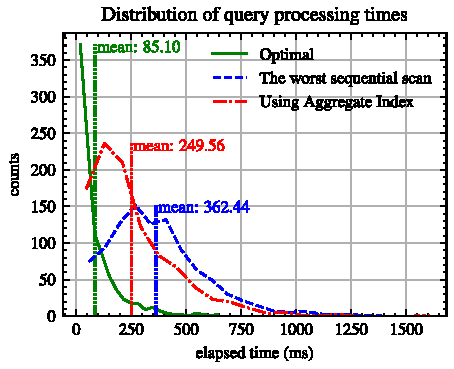
\includegraphics[]{graphics/agg_vs_partitioned_A.pdf}
		\caption{Workload A}
		\label{fig:agg_vs_partitioned_A}
	\end{subfigure}
	\hfill
	\begin{subfigure}{0.45\textwidth}
		\centering
		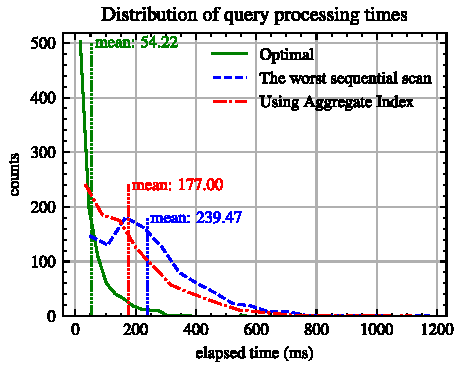
\includegraphics[]{graphics/agg_vs_partitioned_B.pdf}
		\caption{Workload B}
		\label{fig:agg_vs_partitioned_B}
	\end{subfigure}
	\caption{The distribution of query processing times of workload A and B.}
	\label{fig:agg_vs_partitioned_all}
\end{figure}

\subsection{Performance of optimal matching for partial tuple completion}
In this experiment, we examine the performance of optimal matching in three different steps.
In our first step, we set query size to be 10, tuple size to be 200, and edge connectivity density to be 0.1. We compute the optimal matching for 100 times and record the response times. Figure~\ref{fig:tuple_completion_1} shows the histogram of the results.
\begin{figure}[!th]
	\centering
	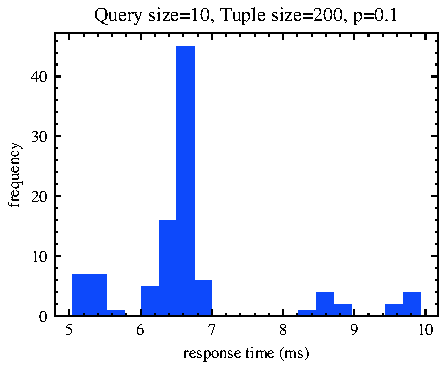
\includegraphics[width=0.6\textwidth]{graphics/tuple_completion_1.pdf}
	\caption{Distribution of optimal matching response times (ms)}
	\label{fig:tuple_completion_1}
\end{figure}
In our second step, we vary edge connectivity densities with the same fixed query size and tuple size as in step one. We repeat the process 100 times and compute the mean response times as results, which are shown in Figure~\ref{fig:tuple_completion_2}.
\begin{figure}[!th]
	\centering
	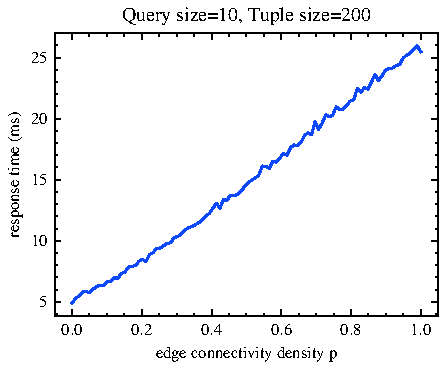
\includegraphics[width=0.6\textwidth]{graphics/tuple_completion_2.pdf}
	\caption{Optimal matching response time (ms) w.r.t. varying edge connectivity densities}
	\label{fig:tuple_completion_2}
\end{figure}
In our last step, we fix the query size and edge connectivity density to be the same as in step one, but change the tuple size so that it goes from 100 to 1,000. Again, we repeat the process for 100 times and compute the mean values. Figure~\ref{fig:tuple_completion_3} shows the results.
\begin{figure}[!th]
	\centering
	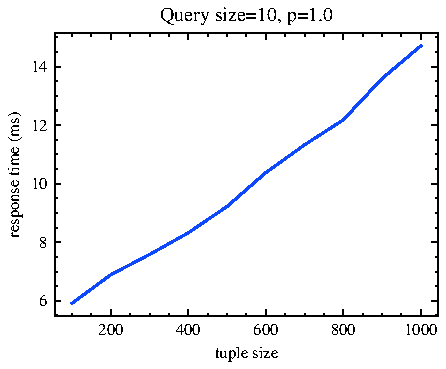
\includegraphics[width=0.6\textwidth]{graphics/tuple_completion_3.pdf}
	\caption{Optimal matching response time (ms) w.r.t. varying tuple sizes}
	\label{fig:tuple_completion_3}
\end{figure}

Our workloads A and B have query sizes of 3 and 5, respectively. The average number of attributes of the 10 datasets is less than 200. 
The experiment results from the above three steps indicate that the response time of optimal matching will be less than 30 milliseconds in our use case. 
The performance cost of optimal matching will not be as significant as that of full-text index lookup. 
Therefore, the majority of our work focuses on how to optimize index lookup using neural networks.

\subsection{Neural network based predictive access}
\label{subsection:nn_experiments}

We evaluate five neural network architectures including MLP, LSTM, Conv1D, Transformer and MLP-Mixer. While all of them can be made into deep networks, or in conjunction with other network architectures, our motivation is to make our models as small as possible so that they can be embedded in a search system.
Therefore, we focus on the minimalist approach to network design.

\subsubsection{Common experimental setup and evaluation metrics}
\noindent{\emph {Evaluation scenarios:}}
 We evaluate models with the following combination of different scenarios in all experiments:
\begin{itemize}
	\item We train the models using different sampling rates of attributes, as described in Section~\ref{subsection:training_data_gen}.
	\item We consider both word-based and 3-gram based training.
	\item We evaluate the performance of index scan using models' predictions
	and compare with the optimal and aggregate index lookup for each query in our query workloads.
\end{itemize}

\noindent{\emph {Tokenization and embedding of texts:}}
The tokens are either words or 3-grams of the values in the partial tuples.  Let $\mathbf{Voc}$ be the vocabulary.  The vocabulary size is determined by the attribute sampling rate during training. The vocabulary sizes are given in Table~\ref{tab:training_vocab_size}. Each token is embedded into $\mathbb{R}^{64}$ by a simple embedding layer that has
$|\mathbf{Voc}|\times 64$ parameters.

\noindent{\emph {Evaluation metrics:}}
We evaluate our models using the following metrics:
\begin{itemize}
\item Top-$k$ classification accuracy: since we know the true relations that contain the partial tuples in our query workloads, we can evaluate the classification accuracy of our model.  The top-$k$ accuracy is defined as the percentage of the correct label among the top-$k$ labels predicted.
\item Index lookup response time using the predicted access pattern: using the likelihoods produced by our model, we can sort the indexes by their likelihoods and access the most likely index first. The scan continues until the true relation is reached.
\end{itemize}

\subsubsection{Multilayer perceptron (MLP)}
\label{subsection:expt_mlp}

\noindent{\emph Description:}

Multilayer perceptron (MLP) is probably the most widely used neural network architecture.  In this experiment, we will test the effectiveness of MLP by itself with a single hidden layer.

\noindent{\emph {Model architecture:}}

\begin{itemize}
    \item Since each query is a sequence of tokens, each query is embedded into
    $\mathbb{R}^{L\times 64}$ where $L$ is the token sequence length.  We use global
    average pooling to generate a flat vector in $\mathbb{R}^{64}$, which is used as the input to the MLP layer.
    \item MLP has one hidden layer of size 100.
    \item We utilize one drop-out layer to prevent overfitting by the large embedding layer.
\end{itemize}

Since we have six sets of training datasets, we have 6 trained MLP models, as shown in Table \ref{tab:trained_mlp_models}.
\begin{table}[!th]
	\centering
	\begin{tabularx}{0.8\textwidth}{|l|X|}
		\hline
		\textbf{Model name} & \textbf{Training dataset} \\ \hline
		mlp100 & 100\% attrs., word-based \\
		mlp100-3gram\ & 100\% attrs., 3-gram based \\ 
		mlp75 & 75\% attrs., word-based \\
		mlp75-3gram & 75\% attrs., 3-gram based \\ 
		mlp50 & 50\% attrs., word-based \\
		mlp50-3gram & 50\% attrs., 3-gram based \\ 
		\hline
	\end{tabularx}
	\caption{MLP model names and corresponding training datasets.}
	\label{tab:trained_mlp_models}
\end{table}

\noindent{\emph Observations:}

\begin{itemize}
	\item The top-1 to top-5 accuracies for all variations of MLP models under the workloads A and B are shown in Figure~\ref{fig:top_k_mlp_all}. Word-based models perform better than 3-gram based models under both workloads, which do not contain misspelled and unknown keywords.
	\item Figure~\ref{fig:mlp_perf_all_A} and Figure~\ref{fig:mlp_perf_all_B} show the distribution of query processing time under the workloads A and B, respectively. Word-based models improve query processing more than 3-gram based models do. In addition, the models trained using partial tuples with less attributes perform better than those trained using partial tuples with more attributes.
\end{itemize}
\begin{figure}[!th]
	\centering
	\begin{subfigure}{0.45\textwidth}
		\centering
%		\includesvg[inkscapelatex=false]{top_k_mlp_A.svg}
		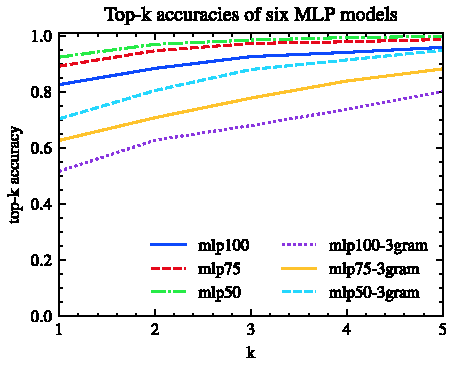
\includegraphics[]{graphics/top_k_mlp_A.pdf}
		\caption{Under the workload A.}
		\label{fig:top_k_mlp_A}
	\end{subfigure}
	\hfill
	\begin{subfigure}{0.45\textwidth}
		\centering
%		\includesvg[inkscapelatex=false]{top_k_mlp_B.svg}
		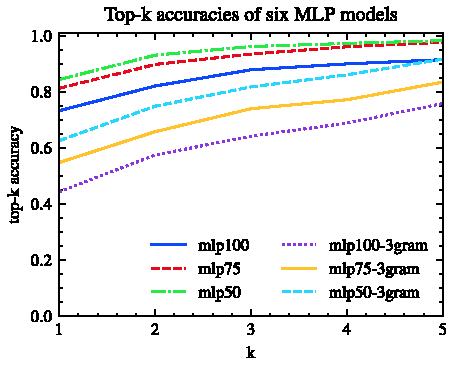
\includegraphics[]{graphics/top_k_mlp_B.pdf}
		\caption{Under the workload B.}
		\label{fig:top_k_mlp_B}
	\end{subfigure}
	\caption{Top-$k$ accuracies of six MLP models under the workload A and B.}
	\label{fig:top_k_mlp_all}
\end{figure}
\begin{figure}[!th]
	\centering
	\begin{subfigure}{0.45\textwidth}
		\begin{subfigure}{\textwidth}
			\centering
%			\includesvg[inkscapelatex=false]{perf_dist_mlp100_A.svg}
			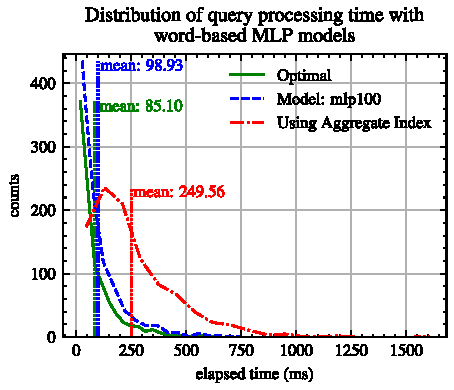
\includegraphics[]{graphics/perf_dist_mlp100_A.pdf}
		\end{subfigure}
		\vfill
		\begin{subfigure}{\textwidth}
			\centering
%			\includesvg[inkscapelatex=false]{perf_dist_mlp75_A.svg}
			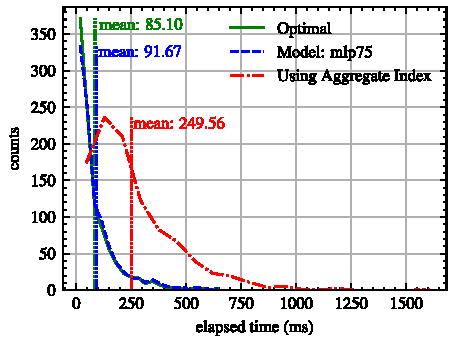
\includegraphics[]{graphics/perf_dist_mlp75_A.pdf}
		\end{subfigure}
		\vfill
		\begin{subfigure}{\textwidth}
			\centering
%			\includesvg[inkscapelatex=false]{perf_dist_mlp50_A.svg}
			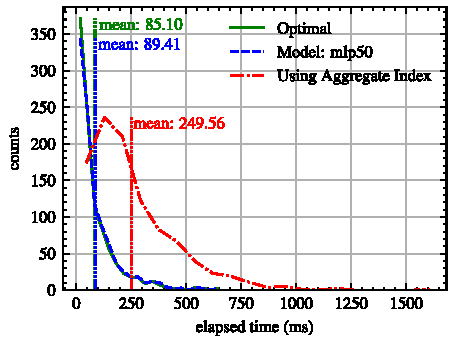
\includegraphics[]{graphics/perf_dist_mlp50_A.pdf}
		\end{subfigure}
		\caption{Word-based MLP models}
	\end{subfigure}
	\hfill
	\begin{subfigure}{0.45\textwidth}
		\begin{subfigure}{\textwidth}
			\centering
%			\includesvg[inkscapelatex=false]{perf_dist_mlp100_3gram_A.svg}
			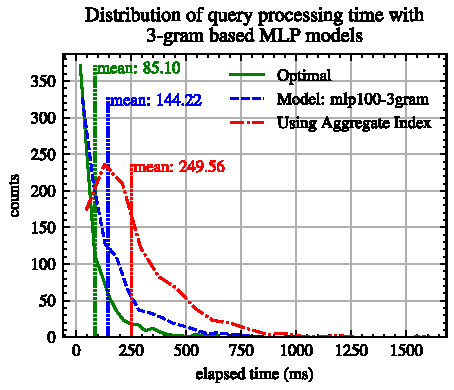
\includegraphics[]{graphics/perf_dist_mlp100_3gram_A.pdf}
		\end{subfigure}
		\vfill
		\begin{subfigure}{\textwidth}
			\centering
%			\includesvg[inkscapelatex=false]{perf_dist_mlp75_3gram_A.svg}
			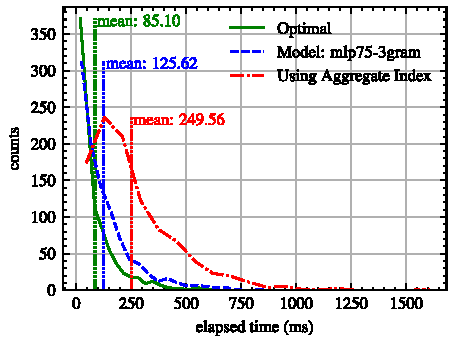
\includegraphics[]{graphics/perf_dist_mlp75_3gram_A.pdf}
		\end{subfigure}
		\vfill
		\begin{subfigure}{\textwidth}
			\centering
%			\includesvg[inkscapelatex=false]{perf_dist_mlp50_3gram_A.svg}
			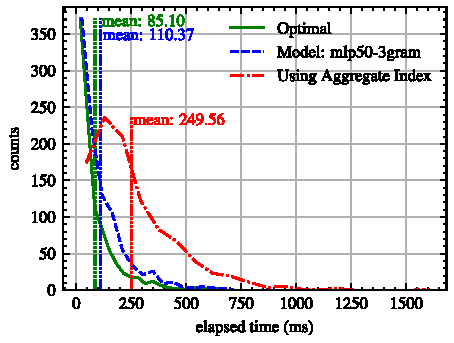
\includegraphics[]{graphics/perf_dist_mlp50_3gram_A.pdf}
		\end{subfigure}
		\caption{3-gram based MLP models}
	\end{subfigure}
	\caption{Distribution of query processing time with MLP models under the workload A.}
	\label{fig:mlp_perf_all_A}
\end{figure}
\begin{figure}[!th]
	\centering
	\begin{subfigure}{0.45\textwidth}
		\begin{subfigure}{\textwidth}
			\centering
%			\includesvg[inkscapelatex=false]{perf_dist_mlp100_B.svg}
			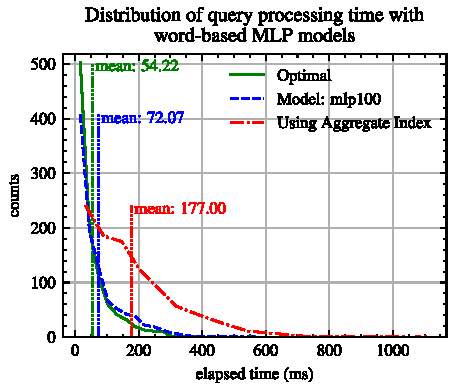
\includegraphics[]{graphics/perf_dist_mlp100_B.pdf}
		\end{subfigure}
		\vfill
		\begin{subfigure}{\textwidth}
			\centering
			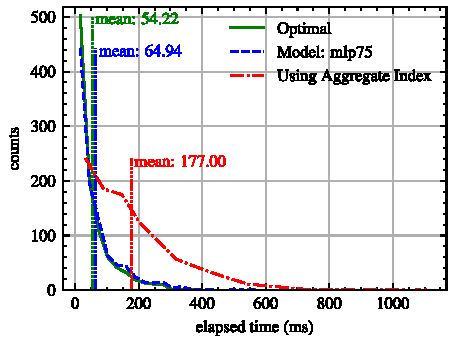
\includegraphics[]{graphics/perf_dist_mlp75_B.pdf}
		\end{subfigure}
		\vfill
		\begin{subfigure}{\textwidth}
			\centering
			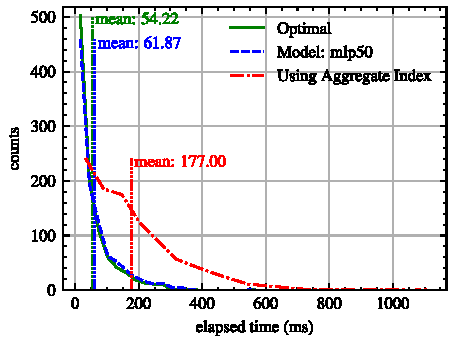
\includegraphics[]{graphics/perf_dist_mlp50_B.pdf}
		\end{subfigure}
		\caption{Word-based MLP models}
	\end{subfigure}
	\hfill
	\begin{subfigure}{0.45\textwidth}
		\begin{subfigure}{\textwidth}
			\centering
			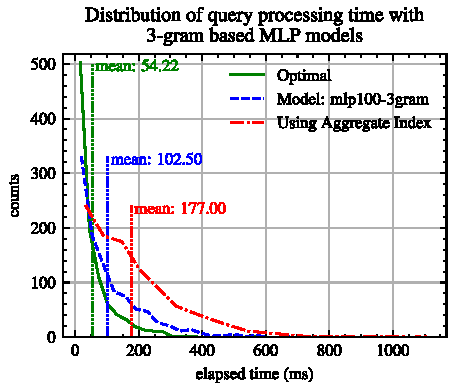
\includegraphics[]{graphics/perf_dist_mlp100_3gram_B.pdf}
		\end{subfigure}
		\vfill
		\begin{subfigure}{\textwidth}
			\centering
			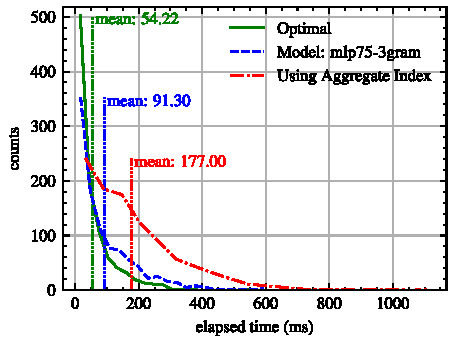
\includegraphics[]{graphics/perf_dist_mlp75_3gram_B.pdf}
		\end{subfigure}
		\vfill
		\begin{subfigure}{\textwidth}
			\centering
			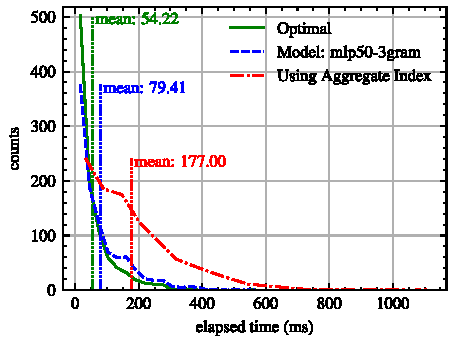
\includegraphics[]{graphics/perf_dist_mlp50_3gram_B.pdf}
		\end{subfigure}
		\caption{3-gram based MLP models}
	\end{subfigure}
	\caption{Distribution of query processing time with MLP models under the workload B.}
	\label{fig:mlp_perf_all_B}
\end{figure}

\subsubsection{Long short-term memory (LSTM)}

\noindent{\emph Description:}

Long short-term memory (LSTM) is a neural network architecture for sequence learning. Even though attributes in a tuple is not considered as a sequence since they are not ordered, the attribute values can be considered as short sequences of tokens. We test how LSTM performs when dealing with relational data in this experiment. Again we apply the minimalist approach to its network design by a single LSTM layer.

\noindent{\emph {Model architecture:}}

\begin{itemize}
	\item Each query is embedded into $\mathbb{R}^{L\times 64}$ where $L$ is the token sequence length, which is used as the input to the LSTM layer.
	\item We apply one drop-out layer to the output of the LSTM layer to prevent overfitting.
	\item The LSTM model has one hidden layer of size 100.
\end{itemize}

\begin{table}[!th]
	\centering
	\begin{tabularx}{0.8\textwidth}{|l|X|}
		\hline
		\textbf{Model name} & \textbf{Training dataset} \\ \hline
		lstm100 & 100\% attrs., word-based \\
		lstm100-3gram & 100\% attrs., 3-gram based \\ 
		lstm75 & 75\% attrs., word-based \\
		lstm75-3gram & 75\% attrs., 3-gram based \\ 
		lstm50 & 50\% attrs., word-based \\
		lstm50-3gram & 50\% attrs., 3-gram based \\ 
		\hline
	\end{tabularx}
	\caption{LSTM model names and corresponding training datasets.}
	\label{tab:trained_lstm_models}
\end{table}

\noindent{\emph Observations:}

\begin{itemize}
	\item The top-1 to top-5 accuracies for all variations of LSTM models under the workloads A and B are shown in Figure~\ref{fig:top_k_lstm_all}. 
	Word-based models perform better than 3-gram based models. When compared to MLP models, LSTM models underperform under both workloads.
	\item Figure~\ref{fig:lstm_perf_all_A} and Figure~\ref{fig:lstm_perf_all_B} show the distribution of query processing time under the workloads A and B, respectively. 
	Word-based models improve query processing more than 3-gram based models do. 
	In addition, similar to MLP models, the models trained using partial tuples with less attributes perform better than those trained using partial tuples with more attributes.
\end{itemize}
\begin{figure}[!th]
	\centering
	\begin{subfigure}{0.45\textwidth}
		\centering
%		\includesvg[inkscapelatex=false]{top_k_lstm_A.svg}
		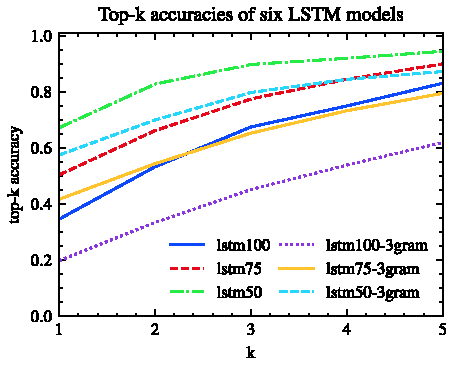
\includegraphics[]{graphics/top_k_lstm_A.pdf}
		\caption{Under the workload A.}
		\label{fig:top_k_lstm_A}
	\end{subfigure}
	\hfill
	\begin{subfigure}{0.45\textwidth}
		\centering
		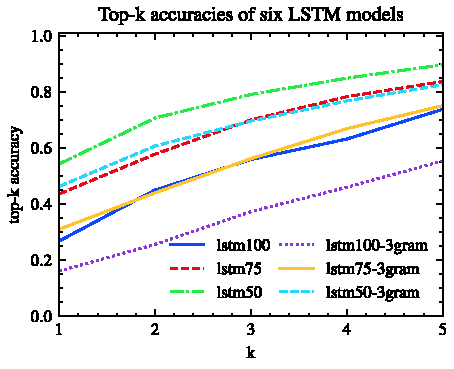
\includegraphics[]{graphics/top_k_lstm_B.pdf}
		\caption{Under the workload B.}
		\label{fig:top_k_lstm_B}
	\end{subfigure}
	\caption{Top-$k$ accuracies of six LSTM models under the workload A and B.}
	\label{fig:top_k_lstm_all}
\end{figure}
\begin{figure}[!th]
	\centering
	\begin{subfigure}{0.45\textwidth}
		\begin{subfigure}{\textwidth}
			\centering
%			\includesvg[inkscapelatex=false]{perf_dist_lstm100_A.svg}
			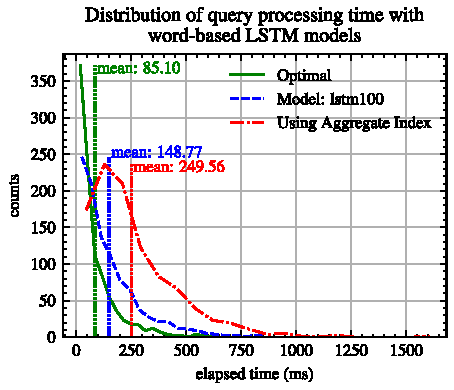
\includegraphics[]{graphics/perf_dist_lstm100_A.pdf}
		\end{subfigure}
		\vfill
		\begin{subfigure}{\textwidth}
			\centering
			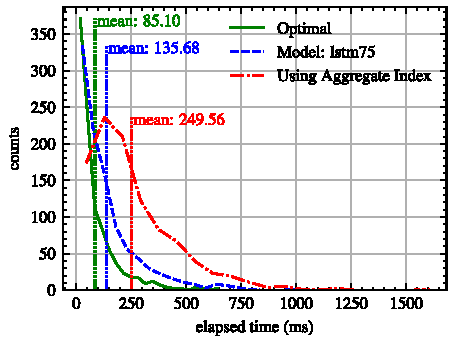
\includegraphics[]{graphics/perf_dist_lstm75_A.pdf}
		\end{subfigure}
		\vfill
		\begin{subfigure}{\textwidth}
			\centering
			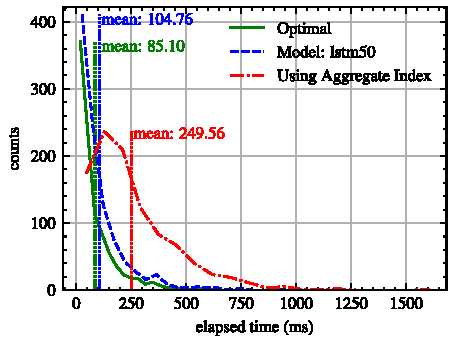
\includegraphics[]{graphics/perf_dist_lstm50_A.pdf}
		\end{subfigure}
		\caption{Word-based LSTM models}
	\end{subfigure}
	\hfill
	\begin{subfigure}{0.45\textwidth}
		\begin{subfigure}{\textwidth}
			\centering
			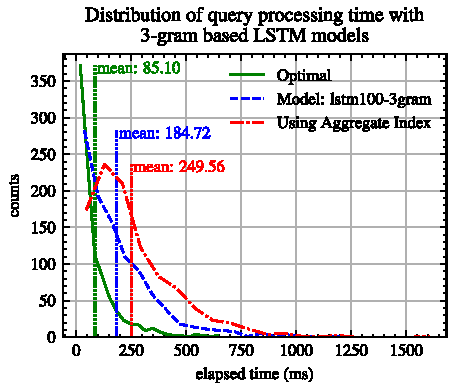
\includegraphics[]{graphics/perf_dist_lstm100_3gram_A.pdf}
		\end{subfigure}
		\vfill
		\begin{subfigure}{\textwidth}
			\centering
			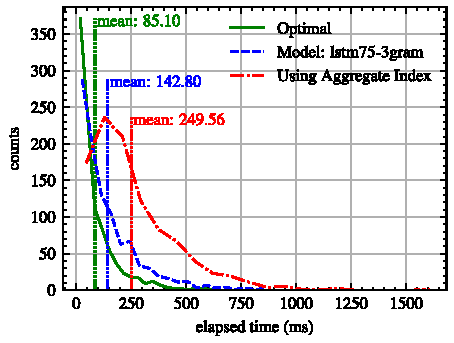
\includegraphics[]{graphics/perf_dist_lstm75_3gram_A.pdf}
		\end{subfigure}
		\vfill
		\begin{subfigure}{\textwidth}
			\centering
			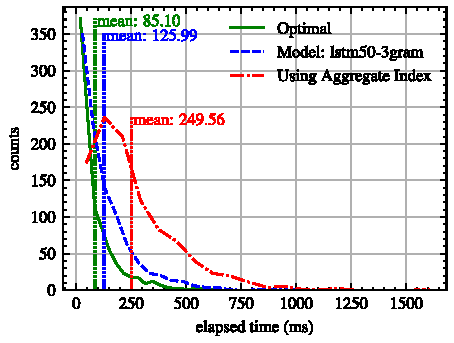
\includegraphics[]{graphics/perf_dist_lstm50_3gram_A.pdf}
		\end{subfigure}
		\caption{3-gram based LSTM models}
	\end{subfigure}
	\caption{Distribution of query processing time with LSTM models under the workload A.}
	\label{fig:lstm_perf_all_A}
\end{figure}
\begin{figure}[!th]
	\centering
	\begin{subfigure}{0.45\textwidth}
		\begin{subfigure}{\textwidth}
			\centering
%			\includesvg[inkscapelatex=false]{perf_dist_lstm100_B.svg}
			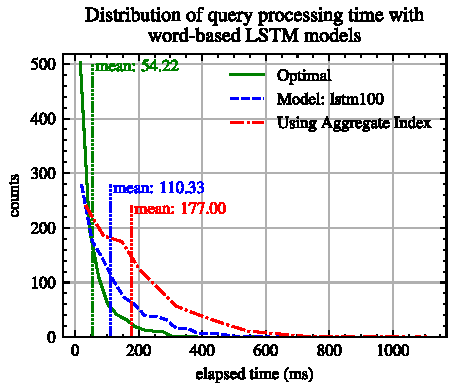
\includegraphics[]{graphics/perf_dist_lstm100_B.pdf}
		\end{subfigure}
		\vfill
		\begin{subfigure}{\textwidth}
			\centering
			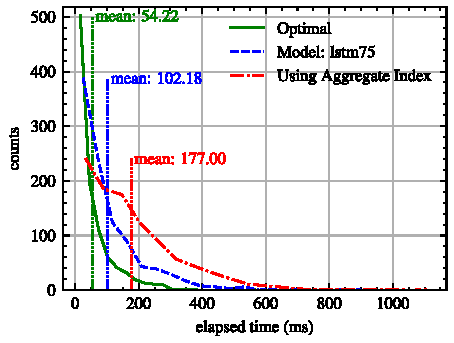
\includegraphics[]{graphics/perf_dist_lstm75_B.pdf}
		\end{subfigure}
		\vfill
		\begin{subfigure}{\textwidth}
			\centering
			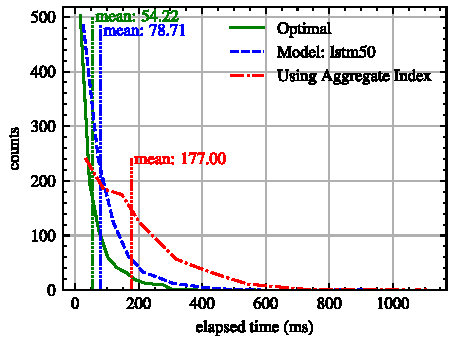
\includegraphics[]{graphics/perf_dist_lstm50_B.pdf}
		\end{subfigure}
		\caption{Word-based LSTM models}
	\end{subfigure}
	\hfill
	\begin{subfigure}{0.45\textwidth}
		\begin{subfigure}{\textwidth}
			\centering
			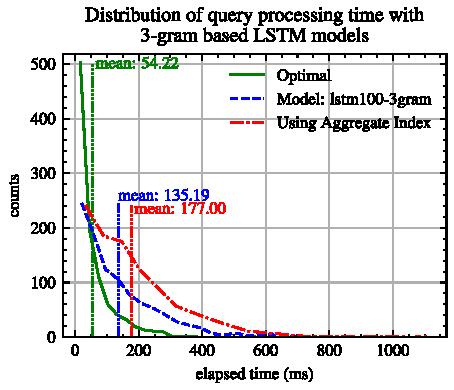
\includegraphics[]{graphics/perf_dist_lstm100_3gram_B.pdf}
		\end{subfigure}
		\vfill
		\begin{subfigure}{\textwidth}
			\centering
			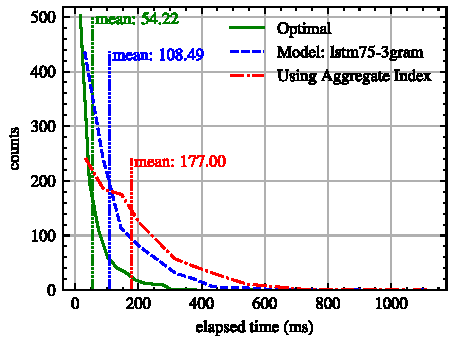
\includegraphics[]{graphics/perf_dist_lstm75_3gram_B.pdf}
		\end{subfigure}
		\vfill
		\begin{subfigure}{\textwidth}
			\centering
			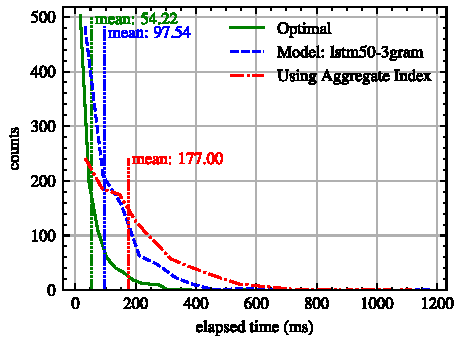
\includegraphics[]{graphics/perf_dist_lstm50_3gram_B.pdf}
		\end{subfigure}
		\caption{3-gram based LSTM models}
	\end{subfigure}
	\caption{Distribution of query processing time with LSTM models under the workload B.}
	\label{fig:lstm_perf_all_B}
\end{figure}

\subsubsection{One dimensional convolution (Conv1D)}

\noindent{\emph Description:}

Another way of doing sequence learning is 1-dimensional convolutional neural networks (Conv1D). Similar to what we do to LSTM, we want to see how Conv1D performs when processing relational data. We also minimize the network structure by using a single Conv1D layer.

\noindent{\emph {Model architecture:}}

\begin{itemize}
	\item Each query is embedded into $\mathbb{R}^{L\times 64}$ where $L$ is the token sequence length, which is used as the input to the Conv1D layer.
	\item The Conv1D layer has 64 kernels with kernel size of 3.
	\item We apply global average pooling to the output of Conv1D layer to generate a flat vector in $\mathbb{R}^{64}$.
	\item We apply one drop-out layer to the flattened vector to prevent overfitting.
\end{itemize}

\begin{table}[!th]
	\centering
	\begin{tabularx}{0.8\textwidth}{|l|X|}
		\hline
		\textbf{Model name} & \textbf{Training dataset} \\ \hline
		conv1d100 & 100\% attrs., word-based \\
		conv1d100-3gram & 100\% attrs., 3-gram based \\ 
		conv1d75 & 75\% attrs., word-based \\
		conv1d75-3gram & 75\% attrs., 3-gram based \\ 
		conv1d50 & 50\% attrs., word-based \\
		conv1d50-3gram & 50\% attrs., 3-gram based \\ 
		\hline
	\end{tabularx}
	\caption{Conv1D model names and corresponding training datasets.}
	\label{tab:trained_conv1d_models}
\end{table}

\noindent{\emph Observations:}

\begin{itemize}
	\item The top-1 to top-5 accuracies for all variations of Conv1D models under the workloads A and B are shown in Figure~\ref{fig:top_k_conv1d_all}. 
	Word-based models perform better than 3-gram based models.
	\item Figure~\ref{fig:conv1d_perf_all_A} and Figure~\ref{fig:conv1d_perf_all_B} show the distribution of query processing time under the workloads A and B, respectively. 
	Word-based models improve query processing more than 3-gram based models do. 
	Under the workload A, the 3-gram based models trained using partial tuples with less attributes perform better than those trained using partial tuples with more attributes, but the word-based models show an opposite relationship.
	Under the workload B, both word-based and 3-gram based models do better when trained using partial tuples with less attributes.
\end{itemize}
\begin{figure}[!th]
	\centering
	\begin{subfigure}{0.45\textwidth}
		\centering
		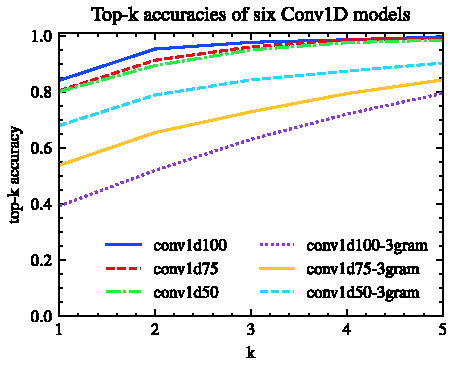
\includegraphics[]{graphics/top_k_conv1d_A.pdf}
		\caption{Under the workload A.}
		\label{fig:top_k_conv1d_A}
	\end{subfigure}
	\hfill
	\begin{subfigure}{0.45\textwidth}
		\centering
		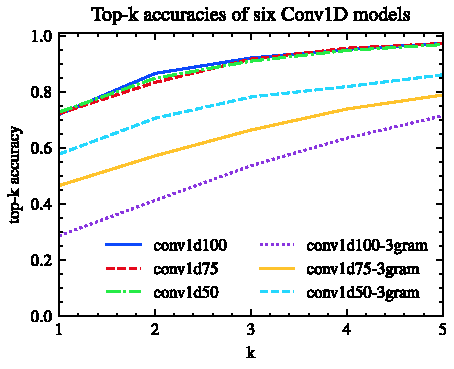
\includegraphics[]{graphics/top_k_conv1d_B.pdf}
		\caption{Under the workload B.}
		\label{fig:top_k_conv1d_B}
	\end{subfigure}
	\caption{Top-$k$ accuracies of six Conv1D models under the workload A and B.}
	\label{fig:top_k_conv1d_all}
\end{figure}
\begin{figure}[!h]
	\centering
	\begin{subfigure}{0.45\textwidth}
		\begin{subfigure}{\textwidth}
			\centering
			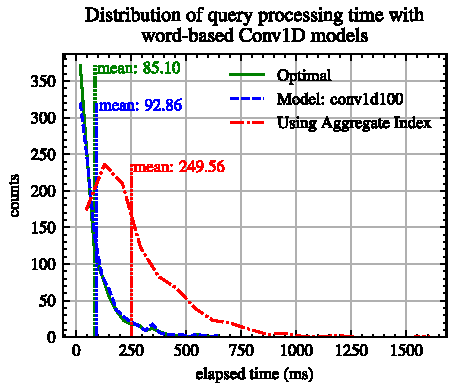
\includegraphics[]{graphics/perf_dist_conv1d100_A.pdf}
		\end{subfigure}
		\vfill
		\begin{subfigure}{\textwidth}
			\centering
			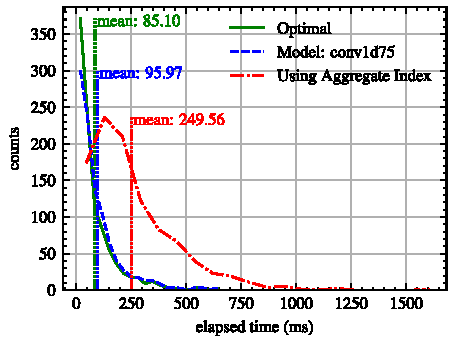
\includegraphics[]{graphics/perf_dist_conv1d75_A.pdf}
		\end{subfigure}
		\vfill
		\begin{subfigure}{\textwidth}
			\centering
			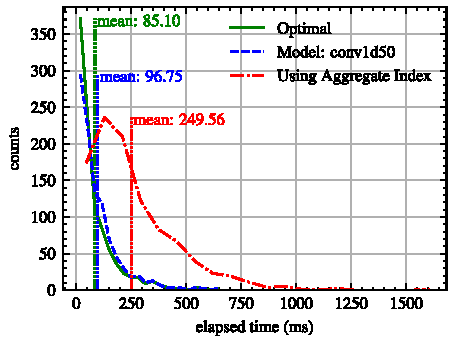
\includegraphics[]{graphics/perf_dist_conv1d50_A.pdf}
		\end{subfigure}
		\caption{Word-based Conv1D models}
	\end{subfigure}
	\hfill
	\begin{subfigure}{0.45\textwidth}
		\begin{subfigure}{\textwidth}
			\centering
			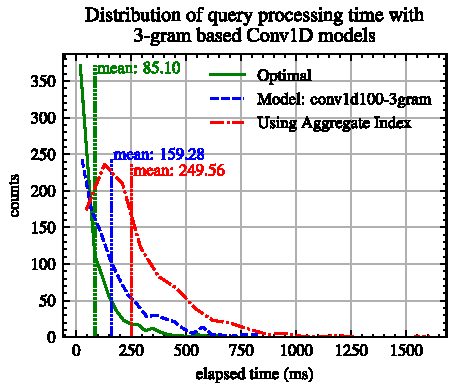
\includegraphics[]{graphics/perf_dist_conv1d100_3gram_A.pdf}
		\end{subfigure}
		\vfill
		\begin{subfigure}{\textwidth}
			\centering
			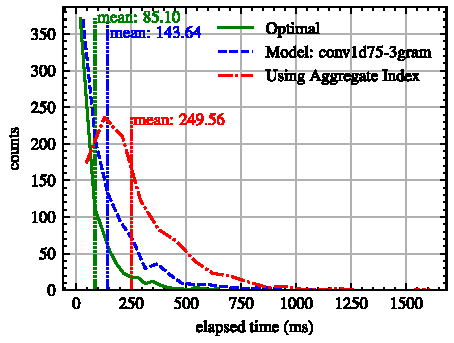
\includegraphics[]{graphics/perf_dist_conv1d75_3gram_A.pdf}
		\end{subfigure}
		\vfill
		\begin{subfigure}{\textwidth}
			\centering
			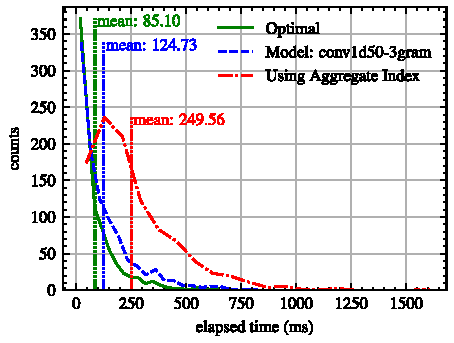
\includegraphics[]{graphics/perf_dist_conv1d50_3gram_A.pdf}
		\end{subfigure}
		\caption{3-gram based Conv1D models}
	\end{subfigure}
	\caption{Distribution of query processing time with Conv1D models under the workload A.}
	\label{fig:conv1d_perf_all_A}
\end{figure}
\begin{figure}[!h]
	\centering
	\begin{subfigure}{0.45\textwidth}
		\begin{subfigure}{\textwidth}
			\centering
			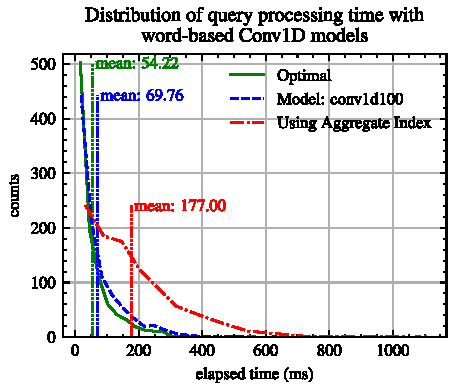
\includegraphics[]{graphics/perf_dist_conv1d100_B.pdf}
		\end{subfigure}
		\vfill
		\begin{subfigure}{\textwidth}
			\centering
			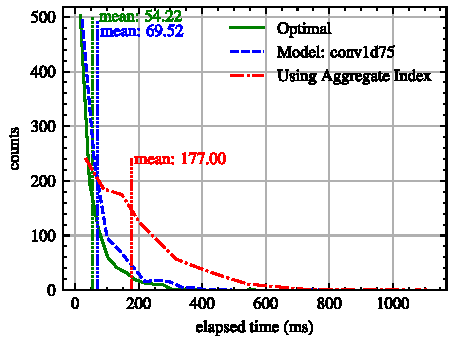
\includegraphics[]{graphics/perf_dist_conv1d75_B.pdf}
		\end{subfigure}
		\vfill
		\begin{subfigure}{\textwidth}
			\centering
			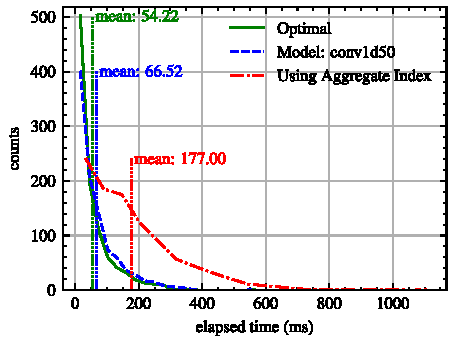
\includegraphics[]{graphics/perf_dist_conv1d50_B.pdf}
		\end{subfigure}
		\caption{Word-based Conv1D models}
	\end{subfigure}
	\hfill
	\begin{subfigure}{0.45\textwidth}
		\begin{subfigure}{\textwidth}
			\centering
			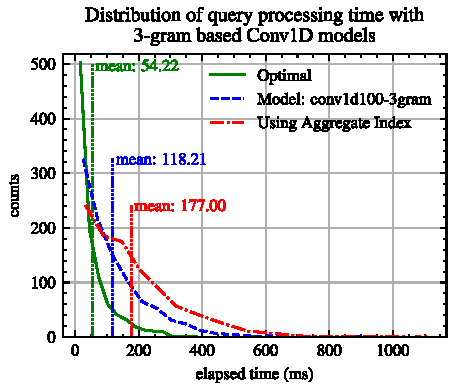
\includegraphics[]{graphics/perf_dist_conv1d100_3gram_B.pdf}
		\end{subfigure}
		\vfill
		\begin{subfigure}{\textwidth}
			\centering
			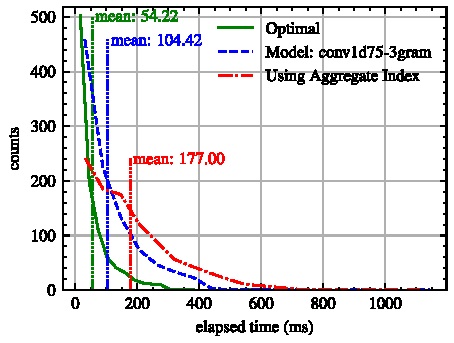
\includegraphics[]{graphics/perf_dist_conv1d75_3gram_B.pdf}
		\end{subfigure}
		\vfill
		\begin{subfigure}{\textwidth}
			\centering
			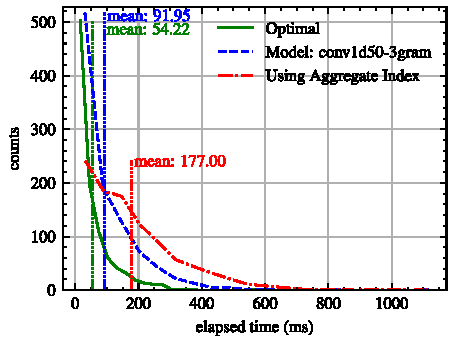
\includegraphics[]{graphics/perf_dist_conv1d50_3gram_B.pdf}
		\end{subfigure}
		\caption{3-gram based Conv1D models}
	\end{subfigure}
	\caption{Distribution of query processing time with Conv1D models under the workload B.}
	\label{fig:conv1d_perf_all_B}
\end{figure}

\subsubsection{Single transformer block}

\noindent{\emph Description:}

The Transformer architecture introduced in the original Transformer paper \cite{DBLP:journals/corr/VaswaniSPUJGKP17} is one of the main advances in natural language processing. In this experiment, we evaluate Transformer architecture for relational data. We largely follow the encoder architecture of the vanilla Transformer presented in the paper \cite{DBLP:journals/corr/VaswaniSPUJGKP17}. However, since our data are relational, we remove positional encoding. In addition, we only create one Transformer block to minimize the model architecture.

\noindent{\emph {Model architecture:}}

\begin{itemize}
	\item Each query is embedded into $\mathbb{R}^{L\times 64}$ where $L$ is the token sequence length, which is used as the input to the Transformer block.
	\item Inside the Transformer block, the attention layer has 4 attention heads. We add an extra drop-out layer after both the attention layer and the feed-forward network to prevent overfitting.
	\item The feed-forward network has a hidden layer of size 64.
	\item We apply global average pooling to the output of the Transformer block to generate a flat vector in $\mathbb{R}^{64}$.
        \item Then we apply a drop-out layer to the flattened vector.
\end{itemize}

\begin{table}[!th]
	\centering
	\begin{tabularx}{0.8\textwidth}{|l|X|}
		\hline
		\textbf{Model name} & \textbf{Training dataset} \\ \hline
		transformer100 & 100\% attrs., word-based \\
		transformer100-3gram & 100\% attrs., 3-gram based \\ 
		transformer75 & 75\% attrs., word-based \\
		transformer75-3gram & 75\% attrs., 3-gram based \\ 
		transformer50 & 50\% attrs., word-based \\
		transformer50-3gram & 50\% attrs., 3-gram based \\ 
		\hline
	\end{tabularx}
	\caption{Transformer model names and corresponding training datasets.}
	\label{tab:trained_transformer_models}
\end{table}
\noindent{\emph Observations:}

\begin{itemize}
	\item The top-1 to top-5 accuracies for all variations of Transformer models under the workloads A and B are shown in Figure~\ref{fig:top_k_transformer_all}. 
	Again, word-based models perform better than 3-gram based models. 
	\item Figure~\ref{fig:transformer_perf_all_A} and Figure~\ref{fig:transformer_perf_all_B} show the distribution of query processing time under the workloads A and B, respectively.
	Word-based models improve query processing more than 3-gram based models do.
	In addition, the models trained using partial tuples with less attributes perform better than those trained using partial tuples with more attributes.
\end{itemize}
\begin{figure}[!th]
	\centering
	\begin{subfigure}{0.45\textwidth}
		\centering
		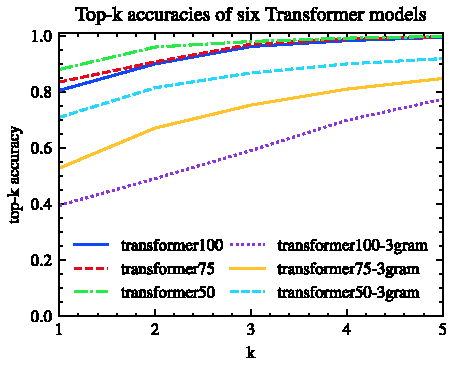
\includegraphics[]{graphics/top_k_transformer_A.pdf}
		\caption{Under the workload A.}
		\label{fig:top_k_transformer_A}
	\end{subfigure}
	\hfill
	\begin{subfigure}{0.45\textwidth}
		\centering
		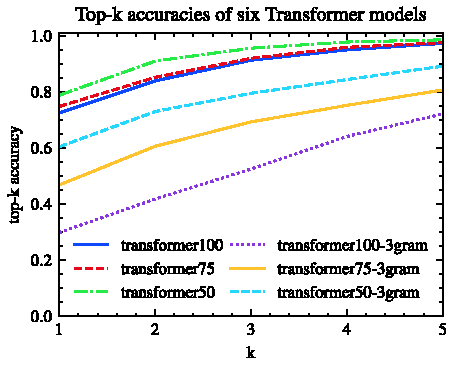
\includegraphics[]{graphics/top_k_transformer_B.pdf}
		\caption{Under the workload B.}
		\label{fig:top_k_transformer_B}
	\end{subfigure}
	\caption{Top-$k$ accuracies of six Transformer models under the workload A and B.}
	\label{fig:top_k_transformer_all}
\end{figure}
\begin{figure}[p]
	\centering
	\begin{subfigure}{0.45\textwidth}
		\begin{subfigure}{\textwidth}
			\centering
			\includegraphics[]{graphics/perf_dist_transformer100_A.pdf}
		\end{subfigure}
		\vfill
		\begin{subfigure}{\textwidth}
			\centering
			\includegraphics[]{graphics/perf_dist_transformer75_A.pdf}
		\end{subfigure}
		\vfill
		\begin{subfigure}{\textwidth}
			\centering
			\includegraphics[]{graphics/perf_dist_transformer50_A.pdf}
		\end{subfigure}
		\caption{Word-based Transformer models}
	\end{subfigure}
	\hfill
	\begin{subfigure}{0.45\textwidth}
		\begin{subfigure}{\textwidth}
			\centering
			\includegraphics[]{graphics/perf_dist_transformer100_3gram_A.pdf}
		\end{subfigure}
		\vfill
		\begin{subfigure}{\textwidth}
			\centering
			\includegraphics[]{graphics/perf_dist_transformer75_3gram_A.pdf}
		\end{subfigure}
		\vfill
		\begin{subfigure}{\textwidth}
			\centering
			\includegraphics[]{graphics/perf_dist_transformer50_3gram_A.pdf}
		\end{subfigure}
		\caption{3-gram based Transformer models}
	\end{subfigure}
	\caption{Distribution of query processing time with Transformer models under the workload A.}
	\label{fig:transformer_perf_all_A}
\end{figure}
\begin{figure}[p]
	\centering
	\begin{subfigure}{0.45\textwidth}
		\begin{subfigure}{\textwidth}
			\centering
			\includegraphics[]{graphics/perf_dist_transformer100_B.pdf}
		\end{subfigure}
		\vfill
		\begin{subfigure}{\textwidth}
			\centering
			\includegraphics[]{graphics/perf_dist_transformer75_B.pdf}
		\end{subfigure}
		\vfill
		\begin{subfigure}{\textwidth}
			\centering
			\includegraphics[]{graphics/perf_dist_transformer50_B.pdf}
		\end{subfigure}
		\caption{Word-based Transformer models}
	\end{subfigure}
	\hfill
	\begin{subfigure}{0.45\textwidth}
		\begin{subfigure}{\textwidth}
			\centering
			\includegraphics[]{graphics/perf_dist_transformer100_3gram_B.pdf}
		\end{subfigure}
		\vfill
		\begin{subfigure}{\textwidth}
			\centering
			\includegraphics[]{graphics/perf_dist_transformer75_3gram_B.pdf}
		\end{subfigure}
		\vfill
		\begin{subfigure}{\textwidth}
			\centering
			\includegraphics[]{graphics/perf_dist_transformer50_3gram_B.pdf}
		\end{subfigure}
		\caption{3-gram based Transformer models}
	\end{subfigure}
	\caption{Distribution of query processing time with Transformer models under the workload B.}
	\label{fig:transformer_perf_all_B}
\end{figure}

\subsubsection{MLP-Mixer}
\label{subsection:expt_mlpmixer}

\noindent{\emph Description:}

MLP-Mixer is an architecture based on MLPs only, which is proposed by Tolstikhin et al. \cite{DBLP:journals/corr/abs-2105-01601}. It is intended for computer vision. However, we want to see whether we could use it for our use case. In this experiment, we modify its architecture for text processing. The same minimalist approach and evaluation scenarios are used as in other experiments.

\noindent{\emph {Model architecture:}}

\begin{itemize}
	\item Each query is embedded into $\mathbb{R}^{L\times 64}$ where $L$ is the token sequence length, which is used as the input to the Mixer Layer.
	\item The Mixer Layer is implemented following the architecture presented in the paper \cite{DBLP:journals/corr/abs-2105-01601}.
	\item Layer normalization is applied to outputs from the Mixer Layer.
	\item We apply global max pooling to the outputs of layer normalization to generate a flat vector in $\mathbb{R}^{64}$, which is used as input to the output layer.
\end{itemize}

\begin{table}[!th]
	\centering
	\begin{tabularx}{0.8\textwidth}{|l|X|}
		\hline
		\textbf{Model name} & \textbf{Training dataset} \\ \hline
		mlpmixer100 & 100\% attrs., word-based \\
		mlpmixer100-3gram & 100\% attrs., 3-gram based \\ 
		mlpmixer75 & 75\% attrs., word-based \\
		mlpmixer75-3gram & 75\% attrs., 3-gram based \\ 
		mlpmixer50 & 50\% attrs., word-based \\
		mlpmixer50-3gram & 50\% attrs., 3-gram based \\ 
		\hline
	\end{tabularx}
	\caption{MLP-Mixer model names and corresponding training datasets.}
	\label{tab:trained_mlpmixer_models}
\end{table}

\noindent{\emph Observations:}

\begin{itemize}
	\item The top-1 to top-5 accuracies for all variations of MLP-Mixer models under the workloads A and B are shown in Figure~\ref{fig:top_k_mlpmixer_all}.
	\item Figure~\ref{fig:mlpmixer_perf_all_A} and Figure~\ref{fig:mlpmixer_perf_all_B} show the distribution of query processing time under the workloads A and B, respectively.
	The word-based models perform slightly better than 3-gram based models, with the exception of two models $\emph mlpmixer75$ and $\emph mlpmixer75$-$3gram$.
	In addition, the models trained using partial tuples with less attributes perform better than those trained using partial tuples with more attributes, 
	with the exception of the model $\emph mlpmixer75$ under the workload B.
\end{itemize}
\begin{figure}[!th]
	\centering
	\begin{subfigure}{0.45\textwidth}
		\centering
		\includegraphics[]{graphics/top_k_mlpmixer_A.pdf}
		\caption{Under the workload A.}
		\label{fig:top_k_mlpmixer_A}
	\end{subfigure}
	\hfill
	\begin{subfigure}{0.45\textwidth}
		\centering
		\includegraphics[]{graphics/top_k_mlpmixer_B.pdf}
		\caption{Under the workload B.}
		\label{fig:top_k_mlpmixer_B}
	\end{subfigure}
	\caption{Top-$k$ accuracies of six MLP-Mixer models under the workload A and B.}
	\label{fig:top_k_mlpmixer_all}
\end{figure}
\begin{figure}[!h]
	\centering
	\begin{subfigure}{0.45\textwidth}
		\begin{subfigure}{\textwidth}
			\centering
			\includegraphics[]{graphics/perf_dist_mlpmixer100_A.pdf}
		\end{subfigure}
		\vfill
		\begin{subfigure}{\textwidth}
			\centering
			\includegraphics[]{graphics/perf_dist_mlpmixer75_A.pdf}
		\end{subfigure}
		\vfill
		\begin{subfigure}{\textwidth}
			\centering
			\includegraphics[]{graphics/perf_dist_mlpmixer50_A.pdf}
		\end{subfigure}
		\caption{Word-based MLP-Mixer models}
	\end{subfigure}
	\hfill
	\begin{subfigure}{0.45\textwidth}
		\begin{subfigure}{\textwidth}
			\centering
			\includegraphics[]{graphics/perf_dist_mlpmixer100_3gram_A.pdf}
		\end{subfigure}
		\vfill
		\begin{subfigure}{\textwidth}
			\centering
			\includegraphics[]{graphics/perf_dist_mlpmixer75_3gram_A.pdf}
		\end{subfigure}
		\vfill
		\begin{subfigure}{\textwidth}
			\centering
			\includegraphics[]{graphics/perf_dist_mlpmixer50_3gram_A.pdf}
		\end{subfigure}
		\caption{3-gram based MLP-Mixer models}
	\end{subfigure}
	\caption{Distribution of query processing time with MLP-Mixer models under the workload A.}
	\label{fig:mlpmixer_perf_all_A}
\end{figure}
\begin{figure}[!h]
	\centering
	\begin{subfigure}{0.45\textwidth}
		\begin{subfigure}{\textwidth}
			\centering
			\includegraphics[]{graphics/perf_dist_mlpmixer100_B.pdf}
		\end{subfigure}
		\vfill
		\begin{subfigure}{\textwidth}
			\centering
			\includegraphics[]{graphics/perf_dist_mlpmixer75_B.pdf}
		\end{subfigure}
		\vfill
		\begin{subfigure}{\textwidth}
			\centering
			\includegraphics[]{graphics/perf_dist_mlpmixer50_B.pdf}
		\end{subfigure}
		\caption{Word-based MLP-Mixer models}
	\end{subfigure}
	\hfill
	\begin{subfigure}{0.45\textwidth}
		\begin{subfigure}{\textwidth}
			\centering
			\includegraphics[]{graphics/perf_dist_mlpmixer100_3gram_B.pdf}
		\end{subfigure}
		\vfill
		\begin{subfigure}{\textwidth}
			\centering
			\includegraphics[]{graphics/perf_dist_mlpmixer75_3gram_B.pdf}
		\end{subfigure}
		\vfill
		\begin{subfigure}{\textwidth}
			\centering
			\includegraphics[]{graphics/perf_dist_mlpmixer50_3gram_B.pdf}
		\end{subfigure}
		\caption{3-gram based MLP-Mixer models}
	\end{subfigure}
	\caption{Distribution of query processing time with MLP-Mixer models under the workload B.}
	\label{fig:mlpmixer_perf_all_B}
\end{figure}

\subsubsection{Comparison of different models}

Based on the observations from Section~\ref{subsection:expt_mlp} to Section~\ref{subsection:expt_mlpmixer}, we have compiled the following table to compare their relative performances with respect to the optimal and the aggregate index lookup under the workload A.

\begin{table}[ht]
    \centering
    \begin{tabularx}{\textwidth}{|l|X||X|X||X|X|X|}
    \hline
    &    \multicolumn{3}{|c|}{Word tokens} & \multicolumn{3}{|c|}{3-gram tokens} \\ \hline
    Model 
        & parameters
        & $\frac{\mathrm{model}}{\mathrm{optimal}}$
        & $\frac{\mathrm{model}}{\mathrm{aggr}}$ 
        & parameters
        & $\frac{\mathrm{model}}{\mathrm{optimal}}$
        & $\frac{\mathrm{model}}{\mathrm{aggr}}$
        \\ \hline
    MLP & 3.02M & {\bf 1.10} & 0.37 & 272K & {\bf 1.49} & 0.51\\
    LSTM & 3.05M & 1.52 & 0.52 & 305K & 1.78 & 0.61 \\
    Conv1D & 3.03M & {\bf 1.12} & 0.38 & 277K & 1.68 & 0.57 \\
    Transformer & 3.09M & {\bf 1.12} & 0.38 & 340K & {\bf 1.66} & 0.57 \\
    MLP Mixer & 3.04M & 1.65 & 0.56 & 287K & {\bf 1.65} & 0.56 \\ \hline
    \end{tabularx}
    \caption{Comparison of models under the workload A with the top-3 measurements highlighted.}
    \label{tab:model-comparison}
\end{table}

The observation supports our proposal of utilizing neural networks to accelerate
index lookup.  As shown in Table~\ref{tab:model-comparison}, many of the models perform well compared to the optimal index lookup, and significantly outperform the aggregate index lookup.

For word based tokens, MLP is only 10\% slower than the optimal index lookup, and outperforms the aggregate index by almost 3 times. The Conv1D and Transformer are only slightly worse than MLP. But the transformer models have larger model sizes. Both LSTM and MLP Mixer do not perform that well when compared to the other three networks.

We realize that we only use one transformer block and one MLP Mixer Layer, respectively.  In our context, we are interested in embedded networks as part of the query processor. Therefore, our focus is limited to small network architectures.

Regarding the model sizes, the main source of parameters is the embedding layer.
Word based tokens produce far more bigger vocabulary, which then requires many more
embedding vectors as model parameters.  The vocabulary of 3-grams is much smaller, and thus produces much more compact models.

Since 3-gram tokens individually capture less information than word-based tokens, we expect the observed performance degradation when using the 3-gram tokens. With that being said, MLP has shown to outperform the aggregate index with twice the performance even for 3-grams.

The value of 3-gram vocabularies becomes more apparent in scenarios with noisy queries.  When query strings contain spelling and other noises at a sub-word level, the two methods of tokenization, i.e., word-based and 3-gram based, behave quite differently.
For word-based tokenization, noisy words will generate out-of-vocabulary (OOV) tokens
which do not contribute to the classification of the network.  However, the 3-gram tokenization can still produce {\em some} 3-gram tokens even for misspelled and unknown words in a query string.  The next section is dedicated to evaluate how well word-based and 3-gram based networks behave in the presence of noisy queries.

\subsection{Impact of noisy queries on models' performance}
\label{subsection:expt_3gram_resiliency}

\noindent{\emph Descriptions:}

In this experiment, we investigate the impact of misspelled words in queries on the models' performance of top-5 accuracy. We simulate the scenario by replacing a randomly selected character in a word with the special character ``\_". For example, the city name \verb|toronto| becomes \verb|to_onto| after mutation. Its 3-gram tokens will be \verb|[__t, _to, to_, o_o, _on, ont, nto, to_, o__]|.

\noindent{\emph {Observations:}}

The impact of noisy queries on models' performance of top-5 accuracy is shown in Figure \ref{fig:acc_degradation_workload_A_all} and \ref{fig:acc_degradation_workload_B_all}  under  the workload A and B, respectively. The performance degradation of word-based models is much faster than that of 3-gram based models. This clearly shows that 3-gram based models are more resilient to query noises.
\begin{figure}[!th]
	\centering
	\begin{subfigure}[t]{0.95\textwidth}
		\includegraphics[]{graphics/acc_degradation_word_based_A.pdf}
		\caption{Word-based models}
		\label{fig:acc_degradation_workload_A_word_based}
	\end{subfigure}
	\vfill
	\begin{subfigure}[t]{0.95\textwidth}
		\includegraphics[]{graphics/acc_degradation_3gram_based_A.pdf}
		\caption{3-gram based models}
		\label{fig:acc_degradation_workload_A_3gram}
	\end{subfigure}
	\caption{Top-5 accuracy degradation of all models under the workload A.}
	\label{fig:acc_degradation_workload_A_all}
\end{figure}
\begin{figure}[!th]
	\centering
	\begin{subfigure}[]{0.95\textwidth}
		\includegraphics[]{graphics/acc_degradation_word_based_B.pdf}
		\caption{Word-based models}
		\label{fig:acc_degradation_workload_B_word_based}
	\end{subfigure}
	\vfill
	\begin{subfigure}[]{0.95\textwidth}
		\includegraphics[]{graphics/acc_degradation_3gram_based_B.pdf}
		\caption{3-gram based models}
		\label{fig:acc_degradation_workload_B_3gram}
	\end{subfigure}
	\caption{Top-5 accuracy degradation of all models under the workload B3.}
	\label{fig:acc_degradation_workload_B_all}
\end{figure}










































\section{Related Work}

\noindent{\bf{Early papers:}} Hristidis and Papakonstantinou \cite{hristidis2002discover} presented DISCOVER, a system that allowed users to submit keyword queries to relational databases without the knowledge of the underlying database schema. DISCOVER processes keyword queries to generate candidate networks of relations and create execution plans to be submitted to RDBMS, which will return search results.
Liu et al. \cite{liu2006effective} proposed an information retrieval (IR) ranking strategy for effective keyword search related to relational databases. The ranking strategy used four normalization factors for computing ranking scores. 
All answers of a query were ranked based on computed ranking scores, and the top-$k$ answers were returned as results.

\noindent{\bf{Extension to include frequent co-occurring term (FCT):}} Tao and Yu \cite{tao2009finding} proposed an operator called frequent co-occurring term (FCT) search, and an algorithm that could solve FCT search effectively without using the conventional keyword search methods. The purpose of FCT search is to extract the terms that most accurately represent a set of keywords, i.e., to discover the concepts closely related to the keywords set.

\noindent{\bf{Survey of keyword search:}} A survey about research on keyword search in relational databases was done by Park and Lee \cite{park2011keyword}. First they listed fundamental characteristics of keyword search in relational databases: an indexing structure, being able to formalize internal queries based on query keywords, being able to correctly constructing candidate answers, and an answer ranking strategy. Then they investigated five research dimensions, including data representation, ranking, efficient processing, query representation, and result presentation. At the end, they pointed out some promising research directions. One of them is efficient top-$k$ query processing. The authors believed that keyword search in relational databases would benefit from advance in top-$k$ query processing techniques.


\noindent{\bf{Interpretation of keywords in query:}} Zeng et al. \cite{zeng2012isearch} presented a framework based on keyword query interpretations. It incorporated human feedback to remove keyword vaguenesses and use a ranking model for query interpretation evaluation afterwards.

\noindent{\bf{Top-$k$ recommendation:}} Meng et al. \cite{meng2017top} presented an approach to solve typical and semantically related queries to a given query. This can help users to explore their query intentions and improve their query formulation.

\noindent{\bf{Index optimization:}} Ding et al. \cite{ding2020alex} presented an updatable learned index called ALEX, an in-memory index structure, for index optimization. ALEX addressed practical issues related to various types of workloads with dynamic updates. RadixSpline \cite{kipf2020radixspline}, another learned index, tackled the issue of index implementation difficulty. RadixSpline offered quick build using a single pass over data while achieving competitive performance.

\noindent{\bf{Query optimization:}} Bao \cite{marcus2022bao} is a learned query optimization system using reinforcement learning. It can learn from mistakes and adapt to dynamic workloads, data, and schema, thus is capable of applying per-query optimization hints.

\noindent{\bf{Cost models for query processing:}} Siddiqui1 et al. \cite{siddiqui2020cost} investigated how to learn cost models from cloud workloads for big data systems. The learned cost models could be integrated with existing query optimizers. Such a query optimizer could make accurate cost predictions, which can improve resource efficiency in big data systems.


\bibliographystyle{plain}
\bibliography{references.bib}
\end{document}
